\documentclass[aspectratio=169,11pt]{beamer}

\usetheme{Madrid}
\usecolortheme{default}
\setbeamertemplate{navigation symbols}{}
\setbeamersize{text margin left=0.6cm,text margin right=0.6cm}%

\usepackage[T1]{fontenc}
\usepackage[utf8]{inputenc}
\usepackage{lmodern}%
\usepackage[scaled=0.92]{helvet}%
\renewcommand{\familydefault}{\sfdefault}
\usepackage{graphicx}
\usepackage{booktabs}
\usepackage{tabularx}
\usepackage{array}
\usepackage{multirow}
\usepackage{amsmath}
\usepackage{amssymb}
\usepackage{ragged2e}
\usepackage{tikz}
\usetikzlibrary{positioning,calc,arrows.meta}
\usepackage{appendixnumberbeamer}

\graphicspath{{figures/}{./}}

\hyphenpenalty=10000 \exhyphenpenalty=10000
\setlength{\emergencystretch}{2em}%

\ifdefined\DeclareUnicodeCharacter%
\DeclareUnicodeCharacter{2248}{\ensuremath{\approx}}
\DeclareUnicodeCharacter{2264}{\ensuremath{\le}}
\DeclareUnicodeCharacter{2265}{\ensuremath{\ge}}
\DeclareUnicodeCharacter{2192}{\ensuremath{\rightarrow}}
\DeclareUnicodeCharacter{2212}{\ensuremath{-}}
\fi

\definecolor{myblue}{RGB}{0,51,102}
\definecolor{myred}{RGB}{153,0,0}
\setbeamercolor{structure}{fg=myblue}
\setbeamercolor{alerted text}{fg=myred}
\colorlet{Navy}{myblue}
\colorlet{Employee}{myblue}%
\colorlet{Employer}{myred}%
\definecolor{Ink}{HTML}{1A1A1A}
\definecolor{Muted}{HTML}{555555}
\definecolor{Rule}{HTML}{A6A6A6}
\definecolor{Soft}{HTML}{EBEBEB}%
\colorlet{SoftBlue}{Soft}
\colorlet{SoftCopper}{Soft}
\setbeamercolor{normal text}{fg=Ink,bg=white}
\setbeamercolor{background canvas}{bg=white}
\setbeamertemplate{background canvas}[default]
\setbeamercolor{frametitle}{fg=white,bg=myblue}

\newcommand{\FsHead}{\fontsize{11.5}{14}\selectfont\bfseries}%
\newcommand{\FsBody}{\fontsize{10.5}{12.8}\selectfont}%
\newcommand{\FsSmall}{\fontsize{10}{12}\selectfont}%
\newcommand{\FsTable}{\fontsize{10}{12.2}\selectfont}%
\newcommand{\FsTableTight}{\fontsize{9.5}{11.6}\selectfont}%
\newcommand{\FsNote}{\fontsize{8.7}{9.8}\selectfont}%
\setbeamerfont{itemize/enumerate body}{size=\fontsize{10.5}{13}\selectfont}
\setbeamerfont{itemize/enumerate subbody}{size=\fontsize{9.5}{12}\selectfont}

\setbeamerfont{frametitle}{size=\fontsize{14.4}{17.3}\selectfont,series=\bfseries}
\makeatletter
\setbeamertemplate{frametitle}{%
  \ifx\insertframesubtitle\@empty\else
    \PackageError{deck}{Frame body read as a frame subtitle}{Put \string\FrameTop\space first in the frame body}\fi
  \nointerlineskip
  \begin{beamercolorbox}[wd=\paperwidth,ht=0.64cm,dp=0.34cm,leftskip=0.6cm,rightskip=0.6cm]{frametitle}%
    \usebeamerfont{frametitle}\insertframetitle
  \end{beamercolorbox}}
\makeatother

\setbeamertemplate{title page}{%
  \centering
  {\color{Navy}\fontsize{24}{28.8}\selectfont\bfseries\inserttitle\par}\vspace{0.25cm}
  {\color{Ink}\fontsize{13}{16}\selectfont\insertsubtitle\par}\vspace{0.40cm}
  {\color{Navy}\rule{3cm}{0.8pt}\par}\vspace{0.40cm}
  {\color{Ink}\fontsize{12}{14.4}\selectfont\bfseries\insertauthor\par}\vspace{0.10cm}
  {\color{Ink}\FsBody\insertinstitute\par}\vspace{0.06cm}
  {\color{Muted}\FsBody\JointWork\par}\vspace{0.50cm}
  {\color{Muted}\fontsize{9.5}{11.4}\selectfont\insertdate\par}}

\setbeamertemplate{itemize items}[circle]
\setbeamertemplate{itemize subitem}[circle]
\setbeamercolor{itemize item}{fg=Navy}
\setbeamercolor{itemize subitem}{fg=Navy}
\setbeamertemplate{enumerate items}[default]
\setbeamerfont{enumerate item}{series=\bfseries}
\setbeamercolor{enumerate item}{fg=Navy}
\setbeamertemplate{blocks}[default]
\setbeamercolor{block title}{fg=Navy,bg=Soft}
\setbeamercolor{block title alerted}{fg=Navy,bg=Soft}
\setbeamercolor{block body}{fg=Ink,bg=Soft}
\setbeamercolor{block body alerted}{fg=Ink,bg=Soft}
\setbeamerfont{block title}{size=\fontsize{11.5}{14}\selectfont,series=\bfseries}
\setbeamerfont{block title alerted}{size=\fontsize{11.5}{14}\selectfont,series=\bfseries}
\setbeamertemplate{block alerted begin}{%
  \par\vskip\medskipamount
  {\color{Navy}\hrule height 0.07cm}\nointerlineskip
  \begin{beamercolorbox}[wd=\textwidth,leftskip=0.25cm,rightskip=0.25cm,ht=0.62cm,dp=0.18cm]{block title alerted}%
    \usebeamerfont*{block title alerted}\insertblocktitle
  \end{beamercolorbox}%
  {\parskip0pt\par}\nointerlineskip
  \usebeamerfont{block body alerted}%
  \begin{beamercolorbox}[wd=\textwidth,leftskip=0.25cm,rightskip=0.25cm,vmode]{block body alerted}%
    \vskip0.02cm}
\setbeamertemplate{block alerted end}{\vskip0.20cm\end{beamercolorbox}\vskip\smallskipamount}

\setbeamercolor{button}{bg=white,fg=Muted}
\setbeamercolor{button border}{fg=Rule}
\setbeamerfont{button}{size=\fontsize{7}{8.4}\selectfont}

\setbeamerfont{page number in head/foot}{size=\fontsize{7}{8.4}\selectfont}
\setbeamercolor{page number in head/foot}{fg=Muted}
\newif\ifinbackup
\inbackupfalse
\setbeamertemplate{footline}{%
  \leavevmode\hbox{%
  \begin{beamercolorbox}[wd=\paperwidth,ht=0.30cm,dp=0.14cm,leftskip=0.6cm,rightskip=0.6cm]{}%
    \usebeamercolor[fg]{page number in head/foot}\usebeamerfont{page number in head/foot}%
    \ifinbackup\hyperlink{B-index}{\textcolor{myblue}{Backup index}}\fi
    \hfill
    \ifinbackup Backup B\insertframenumber\else\insertframenumber\,/\,\inserttotalframenumber\fi
  \end{beamercolorbox}}}

\setlength{\heavyrulewidth}{0.8pt}
\setlength{\lightrulewidth}{0.4pt}
\newcommand{\MainTableStyle}{\FsTable\setlength{\tabcolsep}{4pt}\renewcommand{\arraystretch}{1.15}%
  \setlength{\belowbottomsep}{0.08cm}}
\newcommand{\RowSep}{\addlinespace[3pt]}
\newcommand{\HeadB}[2]{\parbox[b]{#1}{\raggedright\bfseries #2}}%

\tikzset{
  deckcard/.style={fill=Soft,draw=none},
  deckhead/.style={anchor=north west,inner sep=0pt,align=flush left,font=\FsHead,text=#1},
  deckhead/.default=Navy,
  deckbody/.style={anchor=north west,inner sep=0pt,align=flush left,font=\FsBody,text=Ink},
  deckcell/.style={fill=Soft,draw=none,inner xsep=0.08cm,inner ysep=0.03cm,align=center,font=\FsBody,text=Ink},
  deckheld/.style={fill=white,draw=Rule,dashed,line width=0.4pt,align=center,font=\FsSmall,text=Muted},
  deckchip/.style={fill=Soft,draw=none,minimum height=0.55cm,inner xsep=0.12cm,align=center,font=\FsSmall,text=Ink},
  deckdisc/.style={circle,fill=Ink,text=white,inner sep=0pt,minimum size=0.55cm,font=\fontsize{11}{13}\selectfont\bfseries},
  deckcolhead/.style={anchor=base west,inner sep=0pt,font=\FsBody\bfseries},
  deckarrow/.style={-{Stealth[length=1.6mm]},draw=Muted,line width=0.8pt}}
\newcommand{\DeckCard}[5]{\fill[deckcard] (#1,#2) rectangle (#3,#4); \fill[#5] (#1,#2) rectangle (#3,#2-0.07);}

\newcommand{\ap}{\ensuremath{\approx}\,}
\newcommand{\dg}{\textsuperscript{\textdagger}}
\newcommand{\DgNote}{\textsuperscript{\textdagger}Range across two samples: all respondents, and excluding one online panel with less reliable survey answers.}
\newcommand{\DgShort}{\textsuperscript{\textdagger}Range across all respondents and excluding one online panel.}
\newcommand{\TableFont}{\fontsize{8.5}{10}\selectfont}
\newcommand{\Caveat}[1]{\par{\color{Ink}\fontsize{10}{12}\selectfont\bfseries #1\par}\vspace{0.06cm}}

\newcommand{\Takeaway}[1]{%
  \par\vspace{0.04cm}%
  \begin{alertblock}{\fontsize{9.5}{11.4}\selectfont #1}\end{alertblock}}

\newcommand{\PanelTitle}[2]{\par{\color{#1}\fontsize{10}{12}\selectfont\bfseries #2\par}\vspace{0.04cm}}
\newcommand{\BigStat}[3]{%
  {\color{#1}\fontsize{15}{17}\selectfont\bfseries #2\par}%
  {\color{Ink}\fontsize{8.5}{10}\selectfont\RaggedRight #3\par}\vspace{0.06cm}}
\newcommand{\Body}[1]{{\fontsize{9.5}{11.6}\selectfont\RaggedRight #1\par}}

\newif\ifdeckSrc
\newcommand{\FrameTop}{\global\deckSrcfalse\vskip -0.15cm plus 1filll\relax}
\newcommand{\SourceNote}[1]{\par\vskip 0.06cm plus 1filll\relax
  {\color{Muted}\FsNote\raggedright #1\par}\vspace{0.12cm}\global\deckSrctrue}
\newcommand{\DeckNavGlue}{\par\ifdeckSrc\else\vskip 0pt plus 1filll\relax\fi\global\deckSrcfalse}
\newcommand{\Interp}[1]{\par\vspace{0.06cm}{\centering\color{Ink}\FsBody #1\par}}
\newcommand{\BL}[2]{\hyperlink{#1}{\beamergotobutton{#2}}\hspace{0.15cm}\ignorespaces}
\newcommand{\DeckBtnRow}{\usebeamerfont{button}\baselineskip=8.4pt\relax}
\newcommand{\Backups}[1]{\DeckNavGlue{\DeckBtnRow\noindent\hfill#1\unskip\par}}
\makeatletter
\providecommand{\ShortLabels}{}
\newcommand{\bt@target}{}
\newcommand{\bt@set}[1]{%
  \ifdefined\ShortPath
    \@expandtwoargs\in@{,#1,}{,\ShortLabels,}%
    \ifin@\def\bt@target{#1}\else\def\bt@target{B-index}\fi
  \else\def\bt@target{#1}\fi}
\newcommand{\BackTo}[2]{%
  \DeckNavGlue{\DeckBtnRow\noindent\hfill
  \bt@set{#1}\hyperlink{\bt@target}{\beamerreturnbutton{#2}}\par}}
\newcommand{\BackToTwo}[4]{%
  \DeckNavGlue{\DeckBtnRow\noindent\hfill
  \bt@set{#1}\hyperlink{\bt@target}{\beamerreturnbutton{#2}}%
  \hspace{0.15cm}\bt@set{#3}\hyperlink{\bt@target}{\beamerreturnbutton{#4}}\par}}
\makeatother
\AtBeginEnvironment{frame}{\global\deckSrcfalse}
\newcommand{\BI}[2]{\hyperlink{#1}{\textcolor{myblue}{#2}}\par}
\newcommand{\BIi}[2]{\hyperlink{#1}{\textcolor{myblue}{#2}}}
\newcommand{\BH}[1]{\vspace{0.12cm}{\color{Ink}\fontsize{9.5}{11.4}\selectfont\bfseries #1\par}}

\newcommand{\Pend}[1]{\textcolor{red}{#1}}
\newcommand{\Fig}[2]{{\centering\includegraphics[width=\linewidth,height=#2,keepaspectratio]{#1}\par}}
\newcommand{\FigC}[1]{{\centering\includegraphics{#1}\par}}
\setbeamercolor{decision}{fg=white,bg=myblue}
\newcommand{\DecisionBanner}[1]{\par
  \begin{beamercolorbox}[wd=\textwidth,sep=0.10cm,center,rounded=false]{decision}%
    {\fontsize{10.5}{12.6}\selectfont\bfseries #1}\end{beamercolorbox}\par}

\newcommand{\Tab}[1]{{\centering\TableFont\input{tables/#1}\par}}
\newcommand{\BackupFig}[7]{%
  \begin{frame}[t,label=#1]{#2}
    \FrameTop
    \Fig{#3}{#4}
    \SourceNote{#7}
    \BackTo{#5}{#6}
  \end{frame}}
\newcommand{\BackupTab}[6]{%
  \begin{frame}[t,label=#1]{#2}
    \FrameTop
    \Tab{#3}
    \SourceNote{#6}
    \BackTo{#4}{#5}
  \end{frame}}

\title[The Price of Flexibility]{The Price of Flexibility}
\subtitle{What PMEs value, what employers weigh, and where they meet}
\author[Seonghoon Kim]{Seonghoon Kim}
\institute[SMU]{Singapore Management University}
\newcommand{\JointWork}{Joint work with the Singapore National Employers Federation (SNEF)}
\date[January 2027]{Preliminary findings for tripartite discussion \textbar\ January 2027}
\hypersetup{pdftitle={The Price of Flexibility},pdfauthor={Seonghoon Kim},
  pdfsubject={Flexible work arrangements in Singapore: PMEs and employers},
  pdfkeywords={flexible work arrangements; TG-FWAR; choice experiment; PMEs; employers}}

\newcommand{\OptionFrame}[9]{%
  \begin{frame}[t,label=#1]{#2}
    \FrameTop%
  {\fontsize{9}{11}\selectfont
    \noindent{\color{Ink}#3}\par
    \vspace{0.06cm}{\color{Rule}\hrule height 0.4pt}\prevdepth=0pt
    \begin{columns}[T,onlytextwidth]
      \begin{column}{0.54\textwidth}
        \PanelTitle{Navy}{The evidence}
        #4\par
        \vspace{0.12cm}
        \PanelTitle{Navy}{Owner and first step}
        #5\par
      \end{column}
      \begin{column}{0.42\textwidth}
        \PanelTitle{Navy}{Builds on}
        #6\par
        \vspace{0.12cm}
        \PanelTitle{Navy}{What it is not}
        #7\par
        \vspace{0.12cm}
        \PanelTitle{Navy}{What to watch}
        #8\par
      \end{column}
    \end{columns}\par}
    #9
  \end{frame}}

\def\ShortLabels{M-title,M-motivation,M-question,M-framework,M-design,M-pmes,M-why-pmes,M-employers,M-where,M-meet,M-puzzle,M-barriers,M-options,M-conclusion,M-thanks}
\ifdefined\ShortPath
  \includeonlyframes{M-title,M-motivation,M-question,M-framework,M-design,M-pmes,M-why-pmes,M-employers,M-where,M-meet,M-puzzle,M-barriers,M-options,M-conclusion,M-thanks,B-index,B-index-all,B-laboursupply,B-talent,B-triangulation,B-guidelines,B-partners,B-legal,B-intl,B-zones,B-validity,B-sample,B-industry,B-panel,B-governance,B-cards,B-paygaps,B-hedonic,B-methods,B-eqpay,B-landscape,B-setup,B-emp-all,B-remote-commute,B-emp-benchmarks,B-why-pmes,B-emp-groups,B-access,B-emp-robust,B-org-yardstick,B-org-salary,B-why-org,B-org-splits,B-org-concerns,B-org-view,B-industry-note,B-modelfree,B-puzzle,B-pilot,B-flexiload,B-career-who,B-career,B-tgfwar,B-awareness,B-approvals,B-approvals-tab,B-requestrate,B-limits,B-nextsteps,B-followup,B-optA,B-optB,B-optC,B-optD,B-optD-items,B-why-org-tests,B-language,B-org-pct,B-gap,B-ra-gender,B-ra-age,B-ra-care,B-ra-role,B-ra-edu,B-ra-sameside,B-ra-trim}
\fi

\begin{document}

\begin{frame}[plain,label=M-title]
  \titlepage
\end{frame}
\note{[Short path] Colleagues from MOM, NTUC and SNEF: the question for Singapore is no longer whether flexible work exists, but which arrangements can retain PMEs while remaining workable for firms.
In this joint study with SNEF, 1,020 PMEs and 397 people involved in PME hiring or manpower decisions made mirrored choices on a common menu of arrangements.%
The results point to common ground, a role-dependent case, and arrangements that need testing before scaling.
Values in per cent of pay are a measuring rod, not a proposal to lower pay.
The findings are preliminary; we end with a decision for the partners.
[Timing: 130 words a minute plus 15 seconds a slide. Short path, 15 slides, target 17 to 18 minutes: Title, Motivation, Question, Framework, Design, PMEs, Why PMEs, Employers, Where, Meet, Compressed week, Barriers, Options, Conclusion, Thank you. The full deck adds Literature, Data, Estimation, Descriptive, Groups, Robustness, Discussion and Limits.]}

\begin{frame}[t,label=M-motivation]{Flexible work is mainstream; the policy problem is fit}
  \FrameTop
  \FigC{F_motivation}
  \Interp{Aggregate provision does not tell us whether the arrangements offered\\ are the ones workers value and firms can sustain.}
  \SourceNote{\textbf{Source:} MRSD, MOM (Jun 2026). MOM gives no reason for the 2025 fall; 2024 incl.\ newer types: 77.5\%.}%
  \Backups{\BL{B-laboursupply}{Labour supply} \BL{B-guidelines}{Guidelines}}
\end{frame}
\note{[Short path] Flexible work is now mainstream. In 2008, 28 per cent of establishments with 25 or more staff offered a scheduled flexible arrangement; by mid-2024, 73 per cent did.%
The 2025 reading, 66 per cent, comes from MOM's odd-year survey, which gave 68 in 2023; we do not read the change as an effect of the Guidelines.%
With fewer working-age residents per senior, keeping people in work matters more. [Detail: B-laboursupply.]%
But a firm offering one arrangement may not offer the one a worker values, or one the role can sustain.
So the partners' question is no longer how many firms offer flexibility, but which arrangements, for which roles, on what terms; MOM's surveys are well placed to track that.
That points to three open problems.}

\begin{frame}[t,label=M-question]{The open problem is fit, not whether a process exists}
  \FrameTop%
  \noindent
  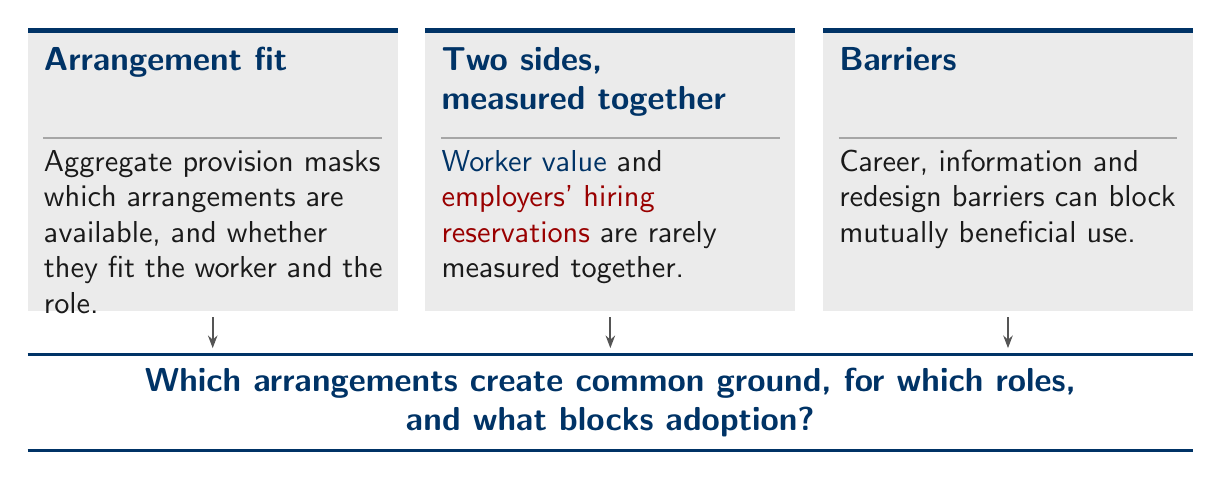
\begin{tikzpicture}[x=1cm,y=1cm,trim left=0cm,trim right=14.8cm]%
    \DeckCard{0}{0}{4.7}{-3.60}{Navy}
    \node[deckhead=Navy] at (0.2,-0.25) {Arrangement fit};
    \draw[Rule,line width=0.6pt] (0.2,-1.40) -- (4.5,-1.40);
    \node[deckbody,text width=4.3cm] at (0.2,-1.55) {Aggregate provision masks which arrangements are available, and whether they fit the worker and the role.};
    \DeckCard{5.05}{0}{9.75}{-3.60}{Navy}
    \node[deckhead=Navy] at (5.25,-0.25) {Two sides,\\measured together};
    \draw[Rule,line width=0.6pt] (5.25,-1.40) -- (9.55,-1.40);
    \node[deckbody,text width=4.3cm] at (5.25,-1.55) {\textcolor{Employee}{Worker value} and \textcolor{Employer}{employers' hiring reservations} are rarely measured together.};
    \DeckCard{10.10}{0}{14.80}{-3.60}{Navy}
    \node[deckhead=Navy] at (10.30,-0.25) {Barriers};
    \draw[Rule,line width=0.6pt] (10.30,-1.40) -- (14.60,-1.40);
    \node[deckbody,text width=4.3cm] at (10.30,-1.55) {Career, information and redesign barriers can block mutually beneficial use.};
    \draw[deckarrow] (2.35,-3.68) -- (2.35,-4.07);
    \draw[deckarrow] (7.40,-3.68) -- (7.40,-4.07);
    \draw[deckarrow] (12.45,-3.68) -- (12.45,-4.07);
    \draw[Navy,line width=0.8pt] (0,-4.15) -- (14.8,-4.15);
    \node[anchor=center,text width=14.4cm,align=center,inner sep=0pt,font=\FsHead,text=Navy] at (7.4,-4.76)
      {Which arrangements create common ground, for which roles,\\and what blocks adoption?};
    \draw[Navy,line width=0.8pt] (0,-5.37) -- (14.8,-5.37);
  \end{tikzpicture}\par
  \Backups{\BL{B-guidelines}{Guidelines} \BL{B-partners}{Partners}}
\end{frame}
\note{[Short path] The Guidelines already set a process for requests. MOM's own survey finds that few who need an arrangement ask formally, a gap MOM attributes to frictions rather than employer resistance.%
What remains open is fit, in three parts.
First, high overall provision can hide which arrangements are on offer, and whether they suit the worker and the role.
Second, few studies measure together how workers value each arrangement and how employers weigh it in hiring; a Polish study is one.%
Third, career worries, unclear terms and the effort of job redesign can block arrangements that would suit both sides; reasons for not asking are rarely measured.
For the partners, the question is which arrangements to make easier to try now, which to tailor by role, which to test before scaling, and what information is missing.
We use a simple map. [Full deck: first, where this sits in the research.]}

\begin{frame}[t,label=M-literature]{Two-sided evidence remains limited}
  \FrameTop%
  {\MainTableStyle\FsTableTight
  \begin{tabularx}{\linewidth}{@{}>{\raggedright\arraybackslash}p{2.6cm}>{\raggedright\arraybackslash}p{2.8cm}>{\raggedright\arraybackslash}X>{\raggedright\arraybackslash}p{3.0cm}@{}}
    \toprule
    & \HeadB{\linewidth}{What existing work measures} & \HeadB{\linewidth}{What it finds \mdseries(not like-for-like)} & \HeadB{\linewidth}{What this study adds}\\
    \midrule
    \textbf{Worker value of WFH}
      & Pay workers would give up for a WFH option
      & About 4--8\% of pay; Singapore 4.8\%, in an online, mostly tertiary-educated sample%
      & Seven arrangements, one design\\%
    \midrule
    \textbf{Employer side and productivity}
      & Employers' expected costs; quits in a firm trial
      & Poland (2023 working paper, hybrid and remote pooled): workers give up 2.9\%, employers expect a 21\% wage cut. Hybrid trial: quits fell by a third%
      & Employers' hiring choices, mirrored with PMEs'\\%
    \midrule
    \textbf{Singapore}
      & Which firms offer FWAs; stated intentions
      & Provision is widespread; FWAs raise stated fertility intentions%
      & Both sides' choices, after the Guidelines took effect\\%
    \bottomrule
  \end{tabularx}\par}
  \SourceNote{\textbf{References:} Mas \& Pallais 2017; Maestas et al.\ 2023; Aksoy et al.\ 2022;\\ Lewandowski et al.\ 2023; Bloom et al.\ 2024; MRSD; Wang \& Dong 2024.}%
  \Backups{\BL{B-emp-benchmarks}{Benchmarks} \BL{B-intl}{Trials}}
\end{frame}
\note{[Full deck only] Three strands frame the study. First, worker valuations: abroad, a work-from-home option is worth about 4 to 8 per cent of pay; a 27-country survey puts Singapore at 4.8 per cent, from an online, mostly tertiary-educated sample.%
Second, the employer side: a 2023 Polish working paper finds workers give up about 3 per cent of pay for remote or hybrid work, while employers expect a 21 per cent wage cut, mostly from expected productivity loss. A six-month trial found hybrid work cut quits by a third.%
[If asked: the published version, ILR Review 2026, reports gaps of about 5 per cent of earnings for hybrid and 25 per cent for fully remote work.]%
Third, Singapore evidence is mostly descriptive. Our study complements this work by observing both sides on a common menu.
Next, a simple map for reading the results.}

\begin{frame}[t,label=M-framework]{Three zones, three policy moves}
  \FrameTop%
  \noindent
  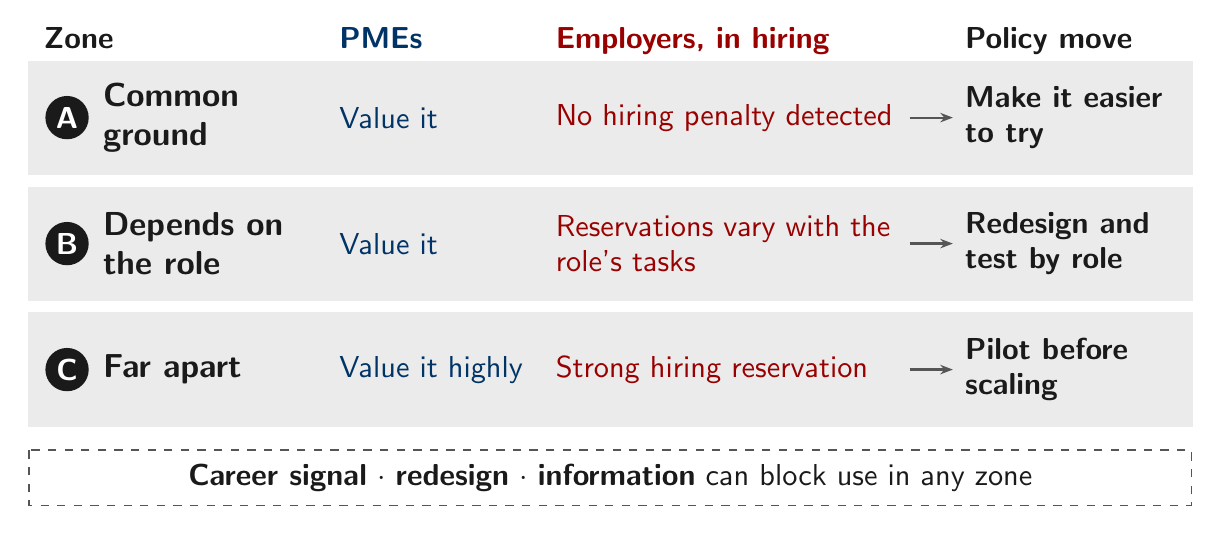
\begin{tikzpicture}[x=1cm,y=1cm,
      band/.style={deckcard},
      zl/.style={deckdisc},
      zn/.style={anchor=west,text width=2.75cm,align=left,inner sep=0pt,font=\FsHead,text=Ink},
      pm/.style={anchor=west,text width=2.6cm,align=left,inner sep=0pt,font=\FsBody,text=Employee},
      em/.style={anchor=west,text width=4.4cm,align=left,inner sep=0pt,font=\FsBody,text=Employer},
      mv/.style={anchor=west,text width=2.8cm,align=left,inner sep=0pt,font=\FsBody\bfseries,text=Ink},
      hdr/.style={deckcolhead},
      arr/.style={deckarrow}]
    \node[hdr,text=Ink] at (0.20,0.15) {Zone};
    \node[hdr,text=Employee] at (3.95,0.15) {PMEs};
    \node[hdr,text=Employer] at (6.70,0.15) {Employers, in hiring};
    \node[hdr,text=Ink] at (11.90,0.15) {Policy move};
    \fill[band] (0,0) rectangle (14.8,-1.45);
    \node[zl] at (0.50,-0.725) {A};
    \node[zn] at (0.95,-0.725) {Common\\ground};
    \node[pm] at (3.95,-0.725) {Value it};
    \node[em] at (6.70,-0.725) {No hiring penalty detected};
    \draw[arr] (11.20,-0.725) -- (11.75,-0.725);
    \node[mv] at (11.90,-0.725) {Make it easier\\to try};
    \fill[band] (0,-1.60) rectangle (14.8,-3.05);
    \node[zl] at (0.50,-2.325) {B};
    \node[zn] at (0.95,-2.325) {Depends on\\the role};
    \node[pm] at (3.95,-2.325) {Value it};
    \node[em] at (6.70,-2.325) {Reservations vary with the role's tasks};
    \draw[arr] (11.20,-2.325) -- (11.75,-2.325);
    \node[mv] at (11.90,-2.325) {Redesign and\\test by role};
    \fill[band] (0,-3.20) rectangle (14.8,-4.65);
    \node[zl] at (0.50,-3.925) {C};
    \node[zn] at (0.95,-3.925) {Far apart};
    \node[pm] at (3.95,-3.925) {Value it highly};
    \node[em] at (6.70,-3.925) {Strong hiring reservation};
    \draw[arr] (11.20,-3.925) -- (11.75,-3.925);
    \node[mv] at (11.90,-3.925) {Pilot before\\scaling};
    \draw[Muted,dashed,line width=0.6pt] (0.02,-4.95) rectangle (14.78,-5.65);
    \node[anchor=center,inner sep=0pt,font=\FsBody,text=Ink] at (7.40,-5.30)
      {\textbf{Career signal} $\cdot$ \textbf{redesign} $\cdot$ \textbf{information} can block use in any zone};
  \end{tikzpicture}\par
  \Backups{\BL{B-methods}{Methods} \BL{B-intl}{Trials}}
\end{frame}
\note{[Short path] We read every result on this map. For each arrangement, we ask how much PMEs value it, and how strongly employers hold back when hiring someone who wants it.
Where PMEs value it and we detect no hiring penalty, there is common ground: firms and SNEF could make it easier to try.
Where reservations depend on the role's tasks, firms can redesign jobs and test role by role.
Where PMEs value it highly but employers hold strong reservations, the sides are far apart: pilot with volunteer firms before scaling.
A reservation may reflect real operating constraints, uncertainty, or what a request seems to signal; hiring choices cannot separate these; a pilot can show whether operating constraints materialise.
In any zone, career signals, redesign and missing information can block use.
Next, how we asked both sides. [Full deck: next, the two surveys.]}

\begin{frame}[t,label=M-data]{Two surveys, unweighted online panels}
  \FrameTop
  \FigC{F_sample_m}
  \Interp{Shares describe surveyed PMEs and firms, not national rates.}
  \SourceNote{\textbf{Source:} this study's PME survey (Aug 2026) and employer survey (Aug--Oct 2026).}
  \Backups{\BL{B-sample}{Sample}\BL{B-panel}{Panels}}
\end{frame}
\note{[Full deck only]
We surveyed both sides of the same labour market.
1,020 citizens and permanent residents in or seeking PME roles answered between 4 and 21 August 2026;%
397 people involved in PME hiring or manpower decisions answered between 12 August and 2 October.%
Both samples come from unweighted online panels, so our shares describe the PMEs and firms we surveyed: MOM's surveys give national rates; ours give the trade-offs.%
We acknowledge that the employer sample leans large: only about one firm in five has 50 or fewer staff.%
SNEF could help recruit smaller member firms, as fresh volunteers, for any next round.%
Next, the choice task.}

\begin{frame}[t,label=M-design]{Mirrored choices on a common FWA menu}
  \FrameTop%
  {\centering
  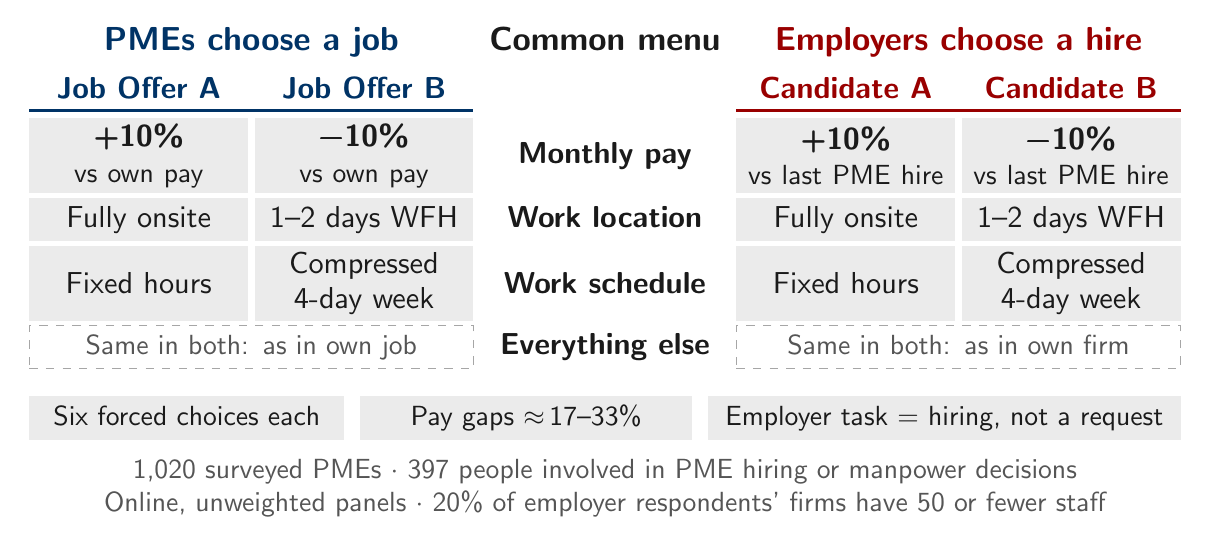
\begin{tikzpicture}[x=1cm,y=1cm,every node/.style={outer sep=0pt},
      hd/.style={anchor=base,inner sep=0pt,font=\FsHead},
      ch/.style={anchor=base west,inner xsep=0.08cm,inner ysep=0pt,minimum width=2.78cm,
        text width=2.62cm,align=center,font=\FsBody\bfseries},
      one/.style={text height=0.27cm,text depth=0.08cm},
      cell/.style={deckcell,anchor=north west,minimum width=2.78cm,text width=2.62cm},
      lab/.style={anchor=north,inner xsep=0.04cm,inner ysep=0.03cm,minimum width=3.18cm,align=center,text=Ink,
        font=\FsBody\bfseries},
      same/.style={deckheld,anchor=north west,inner xsep=0.08cm,inner ysep=0.03cm,minimum width=5.64cm,
        text width=5.48cm,minimum height=0.55cm},
      chip/.style={deckchip,anchor=north west,inner ysep=0.03cm}]
    \node[hd,text=Employee,minimum width=5.64cm] at (2.82,-0.36) {PMEs choose a job};
    \node[hd,text=Ink,minimum width=3.18cm] at (7.31,-0.36) {Common menu};
    \node[hd,text=Employer,minimum width=5.64cm] at (11.80,-0.36) {Employers choose a hire};
    \node[ch,text=Employee] at (0,-0.97) {Job Offer A};
    \node[ch,text=Employee] at (2.86,-0.97) {Job Offer B};
    \node[ch,text=Employer] at (8.98,-0.97) {Candidate A};
    \node[ch,text=Employer] at (11.84,-0.97) {Candidate B};
    \draw[Employee,line width=1.2pt] (0,-1.12) -- (5.64,-1.12);
    \draw[Employer,line width=1.2pt] (8.98,-1.12) -- (14.62,-1.12);
    \node[cell,minimum height=0.95cm] at (0,-1.22) {\textbf{+10\%}\\{\FsSmall vs own pay}};
    \node[cell,minimum height=0.95cm] at (2.86,-1.22) {\textbf{\textminus 10\%}\\{\FsSmall vs own pay}};
    \node[lab,minimum height=0.95cm] at (7.31,-1.22) {Monthly pay};
    \node[cell,minimum height=0.95cm] at (8.98,-1.22) {\textbf{+10\%}\\{\FsSmall vs last PME hire}};
    \node[cell,minimum height=0.95cm] at (11.84,-1.22) {\textbf{\textminus 10\%}\\{\FsSmall vs last PME hire}};
    \node[cell,one,minimum height=0.55cm] at (0,-2.23) {Fully onsite};
    \node[cell,one,minimum height=0.55cm] at (2.86,-2.23) {1--2 days WFH};
    \node[lab,one,minimum height=0.55cm] at (7.31,-2.23) {Work location};
    \node[cell,one,minimum height=0.55cm] at (8.98,-2.23) {Fully onsite};
    \node[cell,one,minimum height=0.55cm] at (11.84,-2.23) {1--2 days WFH};
    \node[cell,minimum height=0.95cm] at (0,-2.84) {Fixed hours};
    \node[cell,minimum height=0.95cm] at (2.86,-2.84) {Compressed\\4-day week};
    \node[lab,minimum height=0.95cm] at (7.31,-2.84) {Work schedule};
    \node[cell,minimum height=0.95cm] at (8.98,-2.84) {Fixed hours};
    \node[cell,minimum height=0.95cm] at (11.84,-2.84) {Compressed\\4-day week};
    \node[same,one] at (0,-3.85) {Same in both: as in own job};
    \node[lab,one,minimum height=0.55cm] at (7.31,-3.85) {Everything else};
    \node[same,one] at (8.98,-3.85) {Same in both: as in own firm};
    \node[chip,one,minimum width=4.00cm,text width=3.76cm] at (0,-4.75) {Six forced choices each};
    \node[chip,one,minimum width=4.22cm,text width=3.98cm] at (4.20,-4.75) {Pay gaps \ap 17--33\%};
    \node[chip,one,minimum width=6.00cm,text width=5.76cm] at (8.62,-4.75) {Employer task = hiring, not a request};
    \node[anchor=north,inner sep=0pt,text width=14.6cm,align=center,text=Muted,font=\FsSmall]
      at (7.31,-5.55) {1,020 surveyed PMEs $\cdot$ 397 people involved in PME hiring or manpower decisions\\%
      Online, unweighted panels $\cdot$ 20\% of employer respondents' firms have 50 or fewer staff};%
  \end{tikzpicture}\par}
  \Backups{\BL{B-cards}{Choice cards}\BL{B-sample}{Sample}}
\end{frame}
\note{[Short path]
Both sides chose from one FWA menu.
We surveyed 1,020 PMEs and 397 people involved in PME hiring or manpower decisions, from unweighted online panels; the firms lean large.%
Each PME chose six times between two job offers; each employer, between two equally qualified candidates.%
Here, offer A pays 10 per cent above the PME's own pay and B 10 per cent below, but B has one to two WFH days and a compressed week: the same hours over four longer days.%
Pay gaps were 17 to 33 per cent by design, so rankings are firmer than prices.%
For employers, this is a hiring choice, not a reply to a request.%
Now the results, starting with PMEs. [Full deck: ``Next, how we turn these choices into values.'']}

\begin{frame}[t,label=M-estimation]{How we turn choices into values}
  \FrameTop%
  {\centering
  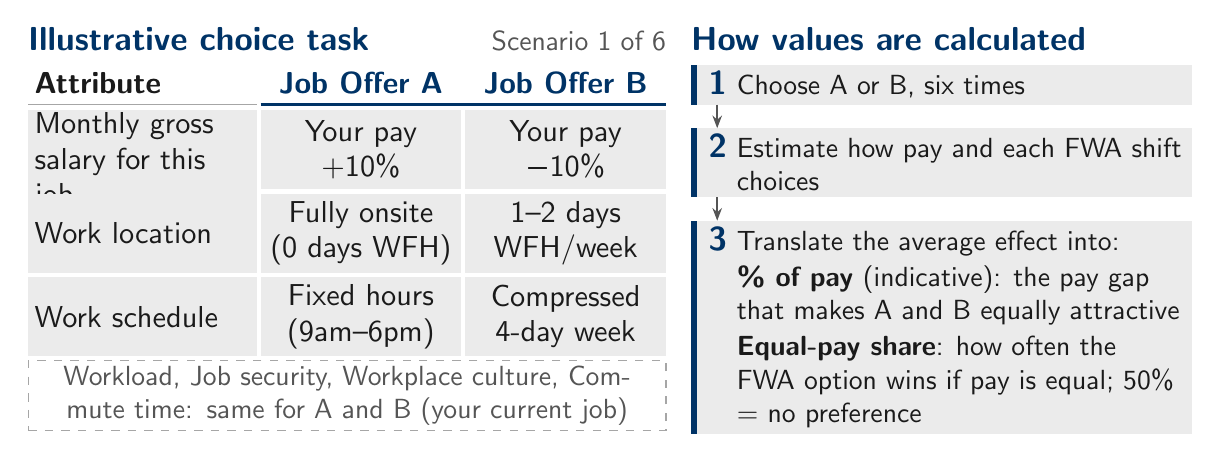
\begin{tikzpicture}[x=1cm,y=1cm,every node/.style={outer sep=0pt},
      lbl/.style={deckcell,anchor=north west,minimum width=2.9cm,text width=2.74cm,align=left},
      hdr/.style={anchor=base west,inner xsep=0.08cm,inner ysep=0pt,minimum width=2.55cm,
        text width=2.39cm,align=center,text=Employee,font=\FsBody\bfseries},
      opt/.style={deckcell,anchor=north west,minimum width=2.55cm,minimum height=1.0cm,text width=2.39cm},
      stepbox/.style={deckcard,anchor=north west,inner xsep=0pt,inner ysep=0.08cm,minimum width=6.36cm,
        text=Ink,font=\FsSmall}]
    \node[deckhead] (hc) at (0,0) {Illustrative choice task};
    \node[anchor=base east,inner sep=0pt,text=Muted,font=\FsSmall] at (8.1,0 |- hc.base) {Scenario 1 of 6};%
    \node[anchor=base west,inner xsep=0.08cm,inner ysep=0pt,text=Ink,font=\FsBody\bfseries]
      at (0,-0.83) {Attribute};
    \node[hdr] at (2.95,-0.83) {Job Offer A};
    \node[hdr] at (5.55,-0.83) {Job Offer B};
    \draw[Employee,line width=1.2pt] (2.95,-0.98) -- (8.1,-0.98);
    \draw[Rule,line width=0.4pt] (0,-0.98) -- (2.9,-0.98);
    \node[lbl,minimum height=1.0cm] at (0,-1.05) {Monthly gross salary for this job};
    \node[opt] at (2.95,-1.05) {Your pay +10\%};
    \node[opt] at (5.55,-1.05) {Your pay \textminus 10\%};
    \node[lbl,minimum height=1.0cm] at (0,-2.11) {Work location};
    \node[opt] at (2.95,-2.11) {Fully onsite\\(0 days WFH)};
    \node[opt] at (5.55,-2.11) {1--2 days\\WFH/week};
    \node[lbl,minimum height=1.0cm] at (0,-3.17) {Work schedule};
    \node[opt] at (2.95,-3.17) {Fixed hours\\(9am--6pm)};
    \node[opt] at (5.55,-3.17) {Compressed\\4-day week};
    \node[deckheld,anchor=north west,inner xsep=0.08cm,inner ysep=0.04cm,minimum width=8.1cm,
      minimum height=0.89cm,text width=7.94cm] at (0,-4.23)
      {Workload, Job security, Workplace culture, Commute time: same for A and B (your current job)};
    \node[deckhead] at (8.42,0) {How values are calculated};
    \node[stepbox] (sA) at (8.42,-0.48)
      {\hspace*{0.22cm}\makebox[0.36cm][l]{\color{Navy}\fontsize{12}{14}\selectfont\bfseries 1}%
      \parbox[t]{5.66cm}{\RaggedRight Choose A or B, six times}\hspace*{0.12cm}};
    \node[stepbox] (sB) at ([yshift=-0.30cm]sA.south west)
      {\hspace*{0.22cm}\makebox[0.36cm][l]{\color{Navy}\fontsize{12}{14}\selectfont\bfseries 2}%
      \parbox[t]{5.66cm}{\RaggedRight Estimate how pay and each FWA shift choices}\hspace*{0.12cm}};%
    \node[stepbox] (sC) at ([yshift=-0.30cm]sB.south west)
      {\hspace*{0.22cm}\makebox[0.36cm][l]{\color{Navy}\fontsize{12}{14}\selectfont\bfseries 3}%
      \parbox[t]{5.66cm}{\RaggedRight Translate the average effect into:\\[0.04cm]%
      \textbf{\% of pay} (indicative): the pay gap that makes A and B equally attractive\\[0.04cm]
      \textbf{Equal-pay share}: how often the FWA option wins if pay is equal; 50\% = no preference}%
      \hspace*{0.12cm}};
    \foreach \s in {sA,sB,sC} {\fill[Navy] (\s.north west) rectangle ([xshift=0.07cm]\s.south west);}
    \draw[deckarrow] ([xshift=0.33cm]sA.south west) -- ([xshift=0.33cm]sB.north west);
    \draw[deckarrow] ([xshift=0.33cm]sB.south west) -- ([xshift=0.33cm]sC.north west);
  \end{tikzpicture}\par}
  \Interp{No equal-pay pair was shown; observed pay gaps were about 17--33\%,\\ so rankings are firmer than prices.}
  \SourceNote{\textbf{Source:} PME questionnaire, Section D. Employers saw the same layout with Candidates A and B.}
  \Backups{\BL{B-methods}{Equations}\BL{B-eqpay}{Equal pay}\BL{B-validity}{Validity}}
\end{frame}
\note{[Full deck only]
This is what a PME saw; employers saw two candidates.%
A statistical model estimates how pay and each arrangement shift the six choices.%
We report two numbers. Per cent of pay is the pay gap that makes the two options equally attractive. The equal-pay share is how often the flexible option wins at equal pay; 50 per cent means no preference.%
We acknowledge that no pair had equal pay and gaps ran from 17 to 33 per cent, so per cent of pay extrapolates.%
MOM, SNEF and NTUC can rely on the rankings; per cent of pay is a rough size, never a proposed pay cut.%
Next, what PMEs and firms do today.}

\begin{frame}[t,label=M-descriptive]{Hybrid is common; compressed weeks are rare}
  \FrameTop
  \FigC{F_landscape_m}
  \Interp{Among surveyed firms, 60\% call 1--2 WFH days typical for PMEs;\\ only 4--6\%\dg\ of surveyed PMEs use a compressed week.}
  \SourceNote{\textbf{Note:} \DgShort\ \textbf{Source:} this study's PME and employer surveys (Aug--Oct 2026).}
  \Backups{\BL{B-landscape}{Landscape}\BL{B-setup}{Pathways}}
\end{frame}
\note{[Full deck only]
Flexible work is already common among the PMEs we surveyed: about seven in ten use at least one arrangement, and 60 per cent of surveyed firms call one to two WFH days typical for their PMEs.%
The compressed week is the exception: four to six per cent of PMEs use one, and about one firm in six offers it.%
These are our samples, not national rates.
More arrangements come through company policy than individual requests, so SNEF could share written FWA policy templates with member firms.%
Is the compressed week rare because PMEs place little value on it, or because employers hesitate? PMEs first.}

\begin{frame}[t,label=M-pmes]{PMEs strongly prefer hybrid work}
  \FrameTop
  \FigC{F_emp_wtp}
  \Interp{The model implies about 7--10\% of pay for hybrid work:\\
    indicative, not a proposed pay cut; observed pay gaps were about 17--33\%.}
  \SourceNote{\textbf{Note:} * Hours change too: not a price of flexibility. Lines: 95\% CIs. \textbf{Source:} PME survey (n = 1,020), Aug 2026 (online panels).}
  \Backups{\BL{B-emp-all}{All estimates}\BL{B-remote-commute}{By commute}}
\end{frame}
\note{[Short path] First, what surveyed PMEs value: the share of monthly pay they would give up for each arrangement, against fully onsite work.
Hybrid work, one to two or three to four WFH days, is worth about 7 to 10 per cent of pay, at or above the upper end of estimates abroad. A compressed week, about 7; staggered hours, about zero; fully remote, against one's own commute, about 13.%
We acknowledge that the pay gaps shown were about 17 to 33 per cent, so these levels are indicative, not a proposed pay cut.%
For firms and SNEF, hybrid options can help attract PMEs alongside pay, not instead of it.
Yet one group chooses WFH less often.
[If asked for dollars: at a median S\$6,000 a month, about S\$400--600; illustrative only.]}%

\begin{frame}[t,label=M-why-pmes]{Career concerns track lower demand for WFH}
  \FrameTop
  \FigC{F_why_pmes}
  \Interp{Consistent with a visibility concern, but asked after the choices\\
    and weaker outside one panel.}
  \SourceNote{\textbf{Note:} Penalty: agrees flexible hours would hurt their career. Associations; lines: 95\% CIs. \textbf{Source:} PME survey (n = 1,020), Aug 2026.}
  \Backups{\BL{B-why-pmes}{All splits}\BL{B-career-who}{Career risk}}
\end{frame}
\note{[Short path] Surveyed PMEs who expect shorter or more flexible hours to hurt their career choose the job with one to two WFH days 52 per cent of the time at equal pay, against 64 per cent for others, statistically significant at the 1 per cent level. For the compressed week, we detect no difference.%
This is consistent with a visibility concern. We acknowledge that the career question was asked after the choices, that part may be noisier answers, and that it is weaker outside one panel.%
For firms and NTUC, appraisal by output could be part of any hybrid pilot.
What do employers weigh in hiring?}

\begin{frame}[t,label=M-employers]{Employers rank fully remote last in hiring}
  \FrameTop
  \FigC{F_org_eqpay}
  \Interp{Ranking, not a salary price: shares of hiring choices at equal pay; 50\% = no preference.\\
    Reservations may reflect operating needs, uncertainty or a candidate signal.}
  \SourceNote{\textbf{Note:} Lines: 95\% CIs. Model-based shares: no pair in the survey had equal pay. \textbf{Source:} employer survey (n = 397), Aug--Oct 2026.}
  \Backups{\BL{B-org-yardstick}{Yardstick}\BL{B-org-salary}{Salary lever}}
\end{frame}
\note{[Short path] Now employers. These are hiring choices between two equally qualified candidates, not responses to a staff request. Each bar is how often the flexible candidate wins at equal salary; 50 per cent means no preference.%
A compressed-week candidate wins 47 per cent: no detectable hiring penalty. One to two WFH days win 40, three to four days 31, and fully remote 23. Each of the three WFH levels is statistically significantly below 50 per cent (p $<$ .001); the compressed week is not (p = .28).%
[For scale: the grey row, a candidate with a high turnover risk, wins 33.6 per cent.]%
Salary moved choices only weakly (the cheaper candidate won 58 per cent): a ranking, not a price.%
Most surveyed firms already use hybrid work: 60 per cent call one to two WFH days typical for PMEs. So a hiring reservation may reflect role needs, uncertainty or a candidate signal, not simply opposition to hybrid work.%
SNEF and member firms could start pilots near the top of this ranking.
Why are some more reserved?}

\begin{frame}[t,label=M-where]{Employer reservations vary with role needs and concerns}
  \FrameTop
  \FigC{F_where_r5}
  \Interp{Preliminary associations under a common pay-slope model;\\
    both items asked after the choices; presence q = .002, creativity q = .43 across 20 splits.}
  \SourceNote{\textbf{Note:} Filled: firms with the need or concern; hollow: other firms. Lines: 95\% CIs. \textbf{Source:} employer survey (n = 397), Aug--Oct 2026.}
  \Backups{\BL{B-why-org}{Tests}\BL{B-org-concerns}{Concerns}\BL{B-org-view}{Employer view}}
\end{frame}
\note{[Short path] Where most PME roles need on-site presence, a candidate wanting one to two WFH days wins 27 per cent at equal pay, against 48 elsewhere. Where firms worry that creativity suffers apart, a fully remote candidate wins 18 per cent, against 29.%
The presence contrast is statistically significant even after correcting for 20 splits (p $<$ .001, q = .002); the creativity contrast is weaker (p = .07, q = .43). Both items were asked after the choices, and a check letting pay sensitivity differ across firms is pending: these are preliminary associations.%
Two in three surveyed employers say FWAs help attract and retain talent; their biggest hurdles are coordination, fairness to staff without FWAs, and productivity.%
Firms, with Job Redesign+ support, could first review which tasks need presence.%
Next, each side against its own 50 per cent.}

\begin{frame}[t,label=M-meet]{Each side, against its own 50\%}%
  \FrameTop
  \FigC{F_meet_r5}
  \Interp{Compressed week: most promising common-ground test;\\ evidence moderate; operating costs unmeasured.}
  \SourceNote{\textbf{Note:} \% of choices at equal pay; 95\% CIs. Zones A--C: descriptive labels. PMEs' remote vs own commute.
    \textbf{Source:} choice experiments with 1,020 surveyed PMEs and 397 employer respondents (Aug--Oct 2026).}
  \Backups{\BL{B-eqpay}{Equal pay} \BL{B-language}{Wording}}
\end{frame}
\note{[Short path] Two panels, two scales. Read each against its own 50 per cent line, meaning no preference; do not compare distances across sides.%
The compressed week, the same hours over four longer days, is the most promising common-ground test: PMEs pick it 58 per cent of the time at equal pay, and employers show no detectable hiring penalty. Evidence is moderate; operating costs are unmeasured.%
One to two WFH days depend on the role. Employers pick candidates wanting three to four days or fully remote well under half the time; these need testing before scaling.%
SNEF and volunteer firms could test the compressed week first. So why is it rare?%
[If asked: the zones are descriptive labels; compressed vs 1--2 days is not statistically significant (p = .09), but 1--2 vs 3--4 days (p $<$ .001) and 3--4 days vs fully remote (p = .003) are.]%
[Full deck: go to M-groups first and ask: does demand differ across PMEs?]}

\begin{frame}[t,label=M-groups]{No subgroup difference detected after correction}
  \FrameTop
  \FigC{F_groups_m}
  \Interp{Non-rejection is not equivalence; groups may still differ.}
  \SourceNote{\textbf{Note:} Lines: 95\% CIs. Fully remote: vs a \textgreater 45 min commute. * Nominal: none of 198 subgroup contrasts survives multiple-testing correction.
    \textbf{Source:} PME choice experiment (1,020 surveyed PMEs).}
  \Backups{\BL{B-emp-groups}{All groups} \BL{B-why-pmes}{All splits}}
\end{frame}
\note{[Full deck only] In every group shown, the interval for choosing a WFH job at equal pay lies above one half.%
None of 198 group contrasts survives correction for multiple testing, and we detect no differences by income, organisation type or tenure.%
We acknowledge that no difference detected is not proof that groups are alike; mothers of young children are a small sample.%
Only the career-concern split survives, as we saw earlier.%
MOM, SNEF and NTUC could therefore treat PME demand for WFH as broad, not niche. Why, then, is the compressed week rare?%
}

\begin{frame}[t,label=M-puzzle]{The compressed week: valued, rarely offered}
  \FrameTop
  \FigC{F_puzzle_r5}
  \Interp{This supports a voluntary, evaluated pilot, not a claim that adoption is costless.}
  \SourceNote{\textbf{Note:} \DgShort\ Surveyed samples, unweighted.
    Design: where only one option had it, the compressed week was the cheaper one in 83\% of PME and 91\% of employer pairs.}
  \Backups{\BL{B-puzzle}{Offering} \BL{B-pilot}{Pilot checklist}}
\end{frame}
\note{[Short path] PMEs value the compressed week and employers show no detectable hiring penalty, yet only about one surveyed firm in six offers it.%
Firms with a written FWA policy offer it more often, 21 against 9 per cent, though a policy may follow offering rather than lead it.%
Where it is available, about one surveyed PME in three takes it up.%
We acknowledge that the design usually made it the cheaper option, and a hiring experiment cannot measure rostering, fatigue or service coverage.%
So the case is for a voluntary, evaluated pilot, not a roll-out: SNEF could recruit volunteer firms to put it on their written menu, with NTUC co-designing safeguards. What happens when PMEs ask?%
}

\begin{frame}[t,label=M-barriers]{We see outcomes for requesters, not why others do not ask}
  \FrameTop
  \FigC{F_barriers_r5}
  \Interp{Career concern covers all surveyed PMEs; refusals cover only reported requesters.\\ We cannot say why others did not ask.}
  \SourceNote{\textbf{Note:} \DgShort\ Grey: the gap between the two.
    \textbf{Source:} PME survey (Aug 2026).}
  \Backups{\BL{B-career-who}{Who expects} \BL{B-approvals-tab}{Approvals}}
\end{frame}
\note{[Short path] Three facts, on different bases. First, across all surveyed PMEs, 37 to 45 per cent expect shorter or more flexible hours to hurt their careers.%
After accounting for who answered, parents of young children are somewhat more likely to expect a career penalty.%
Second, only a quarter to three in ten surveyed junior PMEs are familiar with the Guidelines.%
Third, among PMEs who report a formal request, four to seven per cent report an outright refusal, or about seven to ten per cent once arrangements that apply automatically are set aside, because the request item was partly misread: a selected group, so both are lower bounds.%
We cannot see why PMEs who need an arrangement do not ask. MOM's surveys could add that question, and any pilot needs career safeguards that NTUC could help design.%
One guardrail before the options. These are stated choices from unweighted online panels; rankings are firmer than prices; and the employer splits by role and concern remain preliminary associations.%
[If asked: familiarity goes with more expected career risk, not less.]%
[If asked: among those who asked, 93 to 96 per cent were approved fully or partly, broadly in line with MOM's figure, though definitions differ.]%
[If asked: MOM finds about 6 per cent of FWA users report a setback; that is experience, ours is expectation.]%
[Full deck: M-robust and M-limits come next; the guardrail can be shortened there.]}

\begin{frame}[t,label=M-robust]{Rankings are more credible than levels}
  \FrameTop%
  {\centering\MainTableStyle\input{tables/T_robust_main}\par}
  \Interp{Pay gaps were 17--33\% by design, so levels in \% of pay are model-based;\\ 60 choice situations per side; employer hiring-task validity untested.}
  \SourceNote{\textbf{Source:} choice experiments with 1,020 surveyed PMEs and 397 employer respondents (Aug--Oct 2026).}
  \Backups{\BL{B-validity}{Validity} \BL{B-emp-robust}{Checks}}
\end{frame}
\note{[Full deck only] Which results survive changes to the analysis?%
Dropping the weaker panel, implausible salaries or inattentive respondents, or adding a position term, moves PME values by two points of pay or less; the rankings hold.%
But the pay gaps shown were about 17 to 33 per cent, so values in per cent of pay are model-based.%
We acknowledge two further limits: each side saw only 60 choice situations, so intervals are likely too narrow, and no cited study validates employer hiring choices like these.%
MOM, SNEF and NTUC can therefore act on rankings; prices need a wave with small pay gaps. How do the zones compare?%
}

\begin{frame}[t,label=M-discussion]{What the evidence says about each zone}
  \FrameTop%
  {\centering
  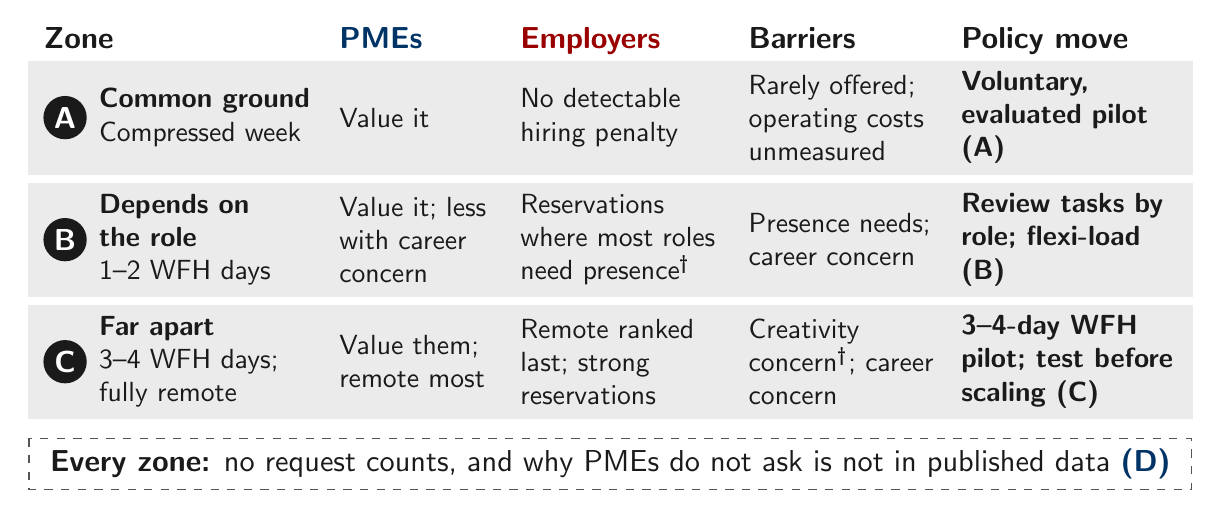
\begin{tikzpicture}[x=1cm,y=1cm,
      zc/.style={deckbody,anchor=west,font=\FsSmall}]
    \node[deckcolhead,text=Ink] at (0.20,0.15) {Zone};
    \node[deckcolhead,text=Employee] at (3.95,0.15) {PMEs};
    \node[deckcolhead,text=Employer] at (6.25,0.15) {Employers};
    \node[deckcolhead,text=Ink] at (9.15,0.15) {Barriers};
    \node[deckcolhead,text=Ink] at (11.85,0.15) {Policy move};
    \fill[deckcard] (0,0) rectangle (14.8,-1.45);
    \fill[deckcard] (0,-1.55) rectangle (14.8,-3.00);
    \fill[deckcard] (0,-3.10) rectangle (14.8,-4.55);
    \node[deckdisc] at (0.475,-0.725) {A};
    \node[zc,text width=2.85cm] at (0.90,-0.725) {\textbf{Common ground}\\ Compressed week};
    \node[zc,text width=2.10cm] at (3.95,-0.725) {Value it};
    \node[zc,text width=2.70cm] at (6.25,-0.725) {No detectable hiring penalty};
    \node[zc,text width=2.50cm] at (9.15,-0.725) {Rarely offered; operating costs unmeasured};
    \node[zc,text width=2.80cm] at (11.85,-0.725) {\textbf{Voluntary, evaluated pilot (A)}};
    \node[deckdisc] at (0.475,-2.275) {B};
    \node[zc,text width=2.85cm] at (0.90,-2.275) {\textbf{Depends on}\\ \textbf{the role}\\ 1--2 WFH days};%
    \node[zc,text width=2.10cm] at (3.95,-2.275) {Value it; less with career concern};
    \node[zc,text width=2.70cm] at (6.25,-2.275) {Reservations where most roles need presence\dg};
    \node[zc,text width=2.50cm] at (9.15,-2.275) {Presence needs; career concern};
    \node[zc,text width=2.80cm] at (11.85,-2.275) {\textbf{Review tasks by role; flexi-load (B)}};
    \node[deckdisc] at (0.475,-3.825) {C};
    \node[zc,text width=2.85cm] at (0.90,-3.825) {\textbf{Far apart}\\ 3--4 WFH days;\\ fully remote};%
    \node[zc,text width=2.10cm] at (3.95,-3.825) {Value them; remote most};
    \node[zc,text width=2.70cm] at (6.25,-3.825) {Remote ranked last; strong reservations};
    \node[zc,text width=2.50cm] at (9.15,-3.825) {Creativity concern\dg; career concern};
    \node[zc,text width=2.80cm] at (11.85,-3.825) {\textbf{3--4-day WFH pilot; test before scaling (C)}};%
    \draw[Muted,dashed,line width=0.6pt] (0.02,-4.80) rectangle (14.78,-5.45);
    \node[anchor=center,inner sep=0pt,font=\FsBody,text=Ink] at (7.40,-5.125)
      {\textbf{Every zone:} no request counts, and why PMEs do not ask is not in published data \textcolor{Navy}{\textbf{(D)}}};
  \end{tikzpicture}\par}
  \SourceNote{\textbf{Note:} \dg\ Preliminary association under a common pay-slope model. \textbf{Source:} PME and employer surveys (Aug--Oct 2026).}
  \Backups{\BL{B-intl}{Trials abroad} \BL{B-puzzle}{Offering}}
\end{frame}
\note{[Full deck only] This map brings the results together and links each zone to an option.%
For the compressed week, PMEs value it and we detect no hiring penalty, yet few surveyed firms offer it, and operating costs are unmeasured; the move is a voluntary, evaluated pilot.%
For one to two WFH days, reservations are concentrated where most roles need presence, a preliminary association, so firms could review tasks by role.%
For three to four days and fully remote work, the two sides are far apart, so pilots come before scaling.%
In every zone, request data are missing. Which options could the partners take up?%
}

\begin{frame}[t,label=M-options]{Options for the partners' decision}
  \FrameTop
  \DecisionBanner{Decision today: one measurement step (we propose D) and one bounded, voluntary pilot (we propose A), each with a lead.}
  \vspace{0.12cm}%
  {\FsTableTight
  \setlength{\tabcolsep}{4pt}
  \renewcommand{\arraystretch}{1.1}
  \begin{tabularx}{\linewidth}{@{}>{\raggedright\arraybackslash}X>{\raggedright\arraybackslash}p{5.0cm}>{\raggedright\arraybackslash}p{3.4cm}@{}}
    \toprule
    \textbf{Option} & \textbf{Owner and first step} & \textbf{Evidence strength}\\
    \midrule
    \hyperlink{B-optA}{\textbf{\textcolor{Navy}{A\enspace Pilot:}}} put compressed weeks on the written menu and test them
      & SNEF and volunteer firms; NTUC: safeguards; TAFEP: guidance
      & Moderate; operating costs unmeasured\\ \addlinespace[2pt]
    \hyperlink{B-optB}{\textbf{\textcolor{Navy}{B\enspace Support:}}} review which tasks need presence; flexi-load where fewer hours, not location, address the need
      & Firms, with Job Redesign+; MOM's PTRG review
      & Moderate; preliminary associations\\ \addlinespace[2pt]
    \hyperlink{B-optC}{\textbf{\textcolor{Navy}{C\enspace Pilot:}}} 3--4-day WFH pilot in roles without presence needs%
      & Volunteer firms; independent evaluation
      & Exploratory\\ \addlinespace[2pt]
    \hyperlink{B-optD}{\textbf{\textcolor{Navy}{D\enspace Measure:}}} why-not-request and partial-approval survey items
      & MRSD checks the items against its survey, with NTUC and SNEF%
      & Gap documented\\
    \bottomrule
  \end{tabularx}\par}
  \Interp{None requires a change to the Guidelines.}
  \Backups{\BL{B-optA}{Option A} \BL{B-optD-items}{Survey items} \BL{B-pilot}{Pilot checklist}}
\end{frame}
\note{[Short path] So to the decision. We ask the partners to choose one measurement step and one bounded, voluntary practice pilot, and to nominate a lead for each. None requires a change to the Guidelines.%
For the pilot, Option A is the most natural: SNEF could recruit volunteer firms to put compressed weeks on their written menu and test them, with NTUC co-designing safeguards, TAFEP providing guidance, and independent evaluation. The evidence is moderate, and operating costs are unmeasured.%
Option B supports implementation: firms could review which tasks need presence, with Job Redesign+, and use flexi-load where fewer hours, not location, address the need.%
Option C, a three-to-four-day WFH pilot in roles without presence needs, is exploratory.%
For measurement, Option D: MRSD, with NTUC and SNEF, could add why-not-request and partial-approval items where its surveys lack them; it adds no reporting duty for firms.%
We close with three messages.%
[Option letters link to B-optA to B-optD. Full deck: M-limits comes next.]}

\begin{frame}[t,label=M-limits]{What we cannot yet say}
  \FrameTop%
  {\MainTableStyle
  \begin{tabularx}{\linewidth}{@{}>{\raggedright\arraybackslash}p{3.0cm}>{\raggedright\arraybackslash}X@{}}
    \toprule
    \textbf{Limit} & \textbf{What it means}\\
    \midrule
    \textbf{Stated choices} & Hypothetical offers; respondents knew SNEF would use the results; rankings firmer than levels\\ \RowSep
    \textbf{Online panels} & Unweighted surveyed PMEs and firms, not national rates; no rank-and-file staff\\ \RowSep
    \textbf{Employer task} & Hiring, not a staff request; may also reflect candidate signals; operating costs unmeasured\\ \RowSep
    \textbf{Few design cells} & 60 choice situations per side; pay gaps 17--33\% by design; intervals likely too narrow\\ \RowSep
    \textbf{Employer splits} & Free-slope check pending: preliminary associations under a common pay-slope model\\ \RowSep
    \textbf{Request item} & Partly misread; why PMEs do not ask is unmeasured\\
    \bottomrule
  \end{tabularx}\par}
  \Backups{\BL{B-limits}{All limits} \BL{B-nextsteps}{Next steps}}
\end{frame}
\note{[Full deck only] We acknowledge six limits. The choices are stated, so rankings are firmer than levels.%
Respondents knew SNEF would use the results, which may invite strategic answers on both sides.%
The panels are online and unweighted, so shares describe surveyed PMEs and firms, not national rates.%
The employer task is a hiring choice, not a reply to a staff request, and does not measure operating costs.%
Each side saw only 60 choice situations, with pay gaps of 17 to 33 per cent, so intervals are likely too narrow.%
The group-specific pay-slope check for the employer splits is pending, so they remain preliminary associations.%
And the request item was partly misread.%
MOM, SNEF and NTUC could each support a next step for these limits. With that, the decision we ask for.%
}

\begin{frame}[t,label=M-conclusion]{The decision we ask of the partners}
  \FrameTop
  \DecisionBanner{Decision sought today: one measurement step and one bounded, voluntary practice pilot, with a lead for each.}
  \vspace{0.20cm}%
  \begin{alertblock}{Take-away messages}
    \begin{enumerate}\setlength{\itemsep}{0.12cm}
      \item PMEs strongly prefer hybrid work: the model implies \textbf{about 7--10\% of pay} (indicative, not a pay cut)
      \item Compressed week: \textbf{most promising common-ground test}; evidence moderate; operating costs unmeasured
      \item Employers rank \textbf{fully remote last} in hiring: a ranking, not a salary price
    \end{enumerate}
  \end{alertblock}
  \Interp{We propose D (why-not and partial-approval items) and A (a compressed-week pilot).}
  \Backups{\BL{B-followup}{Follow-up} \BL{B-optD-items}{Survey items}}
\end{frame}
\note{[Short path] Three messages. First, PMEs strongly prefer hybrid work: the model implies about seven to ten per cent of pay, an indicative value, not a case for lower pay.%
Second, the compressed week, the same hours over four longer days, is the most promising common-ground test: PMEs value it and we detect no hiring penalty, but the evidence is moderate and operating costs are unmeasured.%
Third, employers rank fully remote work last when they hire; that is a ranking, not a salary price.%
We acknowledge that these are stated choices, and the employer splits remain preliminary.%
The policy problem is therefore fit, not aggregate provision: which arrangement, for which role, and what blocks its use. A measurement step would show why PMEs who need an arrangement do not ask; a bounded pilot would show whether the compressed week works in practice.%
For example, MRSD could lead the measurement step, and SNEF a voluntary compressed-week pilot with volunteer firms, with NTUC co-designing safeguards.%
We ask the partners today to choose one measurement step and one bounded, voluntary practice pilot, and to nominate a lead for each.%
[30-second close: PMEs strongly prefer hybrid work, at an indicative seven to ten per cent of pay. The compressed week is the most promising common-ground test, with moderate evidence and unmeasured operating costs, so any pilot needs worker safeguards. Employers rank fully remote last in hiring; that is a ranking, not a price. We ask the partners today to choose one measurement step and one bounded, voluntary practice pilot, and to nominate a lead for each.]
[Follow-up design and consent scope: B-followup.]}

\begin{frame}[plain,label=M-thanks]
  \vskip 0pt plus 1filll
  {\centering
    {\color{Navy}\fontsize{26}{31}\selectfont\bfseries Thank you\par}
    \vspace{0.30cm}
    {\color{Ink}\fontsize{13}{16}\selectfont Questions and discussion\par}
    \vspace{0.40cm}
    {\color{Navy}\rule{3cm}{0.8pt}\par}
    \vspace{0.40cm}
    {\color{Muted}\FsBody Seonghoon Kim $\cdot$ Singapore Management University\\
      Joint work with the Singapore National Employers Federation (SNEF)\par}
  \par}
  \Backups{\BL{B-index}{Backup index}}
  \vspace*{0.58cm}
\end{frame}
\note{[Short path] Thank you; we welcome your questions and comments.}

\appendix
\inbackuptrue

\begin{frame}[t,label=B-index]{Backup index: likely questions}
  \setbeamerfont{itemize/enumerate body}{size=\fontsize{10.5}{12.8}\selectfont}
  \begin{columns}[T,onlytextwidth]
    \begin{column}{0.49\textwidth}
      {\FsHead\color{Ink}Policy and practice\par}
      \begin{itemize}\setlength{\itemsep}{0.12cm}
        \item \BIi{B-tgfwar}{Did the Guidelines change outcomes?}
        \item \BIi{B-legal}{Should FWA requests be legislated?}
        \item \BIi{B-org-view}{Is this a burden for smaller firms?}
        \item \BIi{B-pilot}{How would a compressed-week pilot run?}
        \item \BIi{B-optD-items}{Why do some PMEs not ask?}
        \item \BIi{B-followup}{What next, and with whose consent?}
      \end{itemize}
    \end{column}
    \begin{column}{0.49\textwidth}
      {\FsHead\color{Ink}The evidence\par}
      \begin{itemize}\setlength{\itemsep}{0.12cm}
        \item \BIi{B-career-who}{Is the career risk real?}
        \item \BIi{B-why-org}{Are reservations about roles or concerns?}
        \item \BIi{B-puzzle}{Is the compressed-week result a design artefact?}
        \item \BIi{B-org-salary}{Can employer reservations be priced?}
      \end{itemize}
      \vspace{0.16cm}
      {\FsHead\color{Ink}The study\par}
      \begin{itemize}\setlength{\itemsep}{0.12cm}
        \item \BIi{B-validity}{Do stated choices predict behaviour?}
      \end{itemize}
    \end{column}
  \end{columns}
  \DeckNavGlue\noindent\hfill{\usebeamerfont{button}\hyperlink{B-index-all}{\beamergotobutton{Full backup index}}\hspace{0.15cm}\hyperlink{M-conclusion}{\beamerreturnbutton{Conclusion}}\hspace{0.15cm}\hyperlink{M-thanks}{\beamerreturnbutton{Thank you}}}\par
\end{frame}

\begin{frame}[t,label=B-index-all]{Full backup index}
  \fontsize{9}{10.5}\selectfont
  \begin{columns}[T,onlytextwidth]
    \begin{column}{0.32\textwidth}
      \BH{Motivation and question}
      \mbox{\BIi{B-laboursupply}{Labour supply}}\enspace\textcolor{Muted}{$\cdot$}\enspace \mbox{\BIi{B-talent}{Talent}}\par
      \mbox{\BIi{B-triangulation}{Partners' evidence}}\enspace\textcolor{Muted}{$\cdot$}\enspace \mbox{\BIi{B-guidelines}{Guidelines}}\par
      \mbox{\BIi{B-partners}{Partner positions}}\enspace\textcolor{Muted}{$\cdot$}\enspace \mbox{\BIi{B-legal}{Abroad}}\par
      \BH{Framework}
      \mbox{\BIi{B-intl}{Evidence elsewhere}}\enspace\textcolor{Muted}{$\cdot$}\enspace \mbox{\BIi{B-zones}{Zone rules}}\par
      \BI{B-validity}{Validity of stated choices}
      \BH{Data and design}
      \mbox{\BIi{B-sample}{Sample}}\enspace\textcolor{Muted}{$\cdot$}\enspace \mbox{\BIi{B-industry}{Industries}}\enspace\textcolor{Muted}{$\cdot$}\enspace \mbox{\BIi{B-panel}{Panels}}\par
      \mbox{\BIi{B-governance}{Governance}}\enspace\textcolor{Muted}{$\cdot$}\enspace \mbox{\BIi{B-cards}{Choice cards}}\par
      \mbox{\BIi{B-paygaps}{Pay gaps}}\enspace\textcolor{Muted}{$\cdot$}\enspace \mbox{\BIi{B-hedonic}{Why not pay data}}\par
      \BH{Method}
      \mbox{\BIi{B-methods}{Equations}}\enspace\textcolor{Muted}{$\cdot$}\enspace \mbox{\BIi{B-eqpay}{Equal-pay shares}}\par
      \BH{Practice today}
      \mbox{\BIi{B-landscape}{Landscape}}\enspace\textcolor{Muted}{$\cdot$}\enspace \mbox{\BIi{B-setup}{Pathways}}\par
    \end{column}
    \begin{column}{0.35\textwidth}
      \BH{PMEs}
      \mbox{\BIi{B-emp-all}{All estimates}}\enspace\textcolor{Muted}{$\cdot$}\enspace \mbox{\BIi{B-remote-commute}{Commute}}\par
      \mbox{\BIi{B-emp-benchmarks}{Benchmarks}}\enspace\textcolor{Muted}{$\cdot$}\enspace \mbox{\BIi{B-why-pmes}{All splits}}\par
      \mbox{\BIi{B-emp-groups}{By group}}\enspace\textcolor{Muted}{$\cdot$}\enspace \mbox{\BIi{B-access}{Access}}\enspace\textcolor{Muted}{$\cdot$}\enspace \mbox{\BIi{B-emp-robust}{Checks}}\par
      \BH{Employers}
      \mbox{\BIi{B-org-yardstick}{Yardstick}}\enspace\textcolor{Muted}{$\cdot$}\enspace \mbox{\BIi{B-org-salary}{Salary lever}}\par
      \mbox{\BIi{B-why-org}{Roles and concerns}}\enspace\textcolor{Muted}{$\cdot$}\enspace \mbox{\BIi{B-org-splits}{Splits chart}}\par
      \mbox{\BIi{B-org-concerns}{Concerns}}\enspace\textcolor{Muted}{$\cdot$}\enspace \mbox{\BIi{B-org-view}{Own view; SMEs}}\par
      \BI{B-industry-note}{No industry split}
      \BH{Where the sides meet}
      \mbox{\BIi{B-modelfree}{Raw choices}}\enspace\textcolor{Muted}{$\cdot$}\enspace \mbox{\BIi{B-puzzle}{Compressed week}}\par
      \mbox{\BIi{B-pilot}{Pilot checklist}}\enspace\textcolor{Muted}{$\cdot$}\enspace \mbox{\BIi{B-flexiload}{Flexi-load}}\par
      \BH{Barriers}
      \mbox{\BIi{B-career-who}{Who expects it}}\enspace\textcolor{Muted}{$\cdot$}\enspace \mbox{\BIi{B-career}{Career risk}}\par
      \mbox{\BIi{B-tgfwar}{On the Guidelines}}\enspace\textcolor{Muted}{$\cdot$}\enspace \mbox{\BIi{B-awareness}{Awareness}}\par
      \mbox{\BIi{B-approvals}{Approvals}}\enspace\textcolor{Muted}{$\cdot$}\enspace \mbox{\BIi{B-approvals-tab}{Outcomes}}\enspace\textcolor{Muted}{$\cdot$}\enspace \mbox{\BIi{B-requestrate}{Request rate}}\par
    \end{column}
    \begin{column}{0.29\textwidth}
      \BH{Limits and next steps}
      \mbox{\BIi{B-limits}{Limits}}\enspace\textcolor{Muted}{$\cdot$}\enspace \mbox{\BIi{B-nextsteps}{Next steps}}\enspace\textcolor{Muted}{$\cdot$}\enspace \mbox{\BIi{B-followup}{Follow-up}}\par
      \BH{Options}
      \mbox{\BIi{B-optA}{Option A}}\enspace\BIi{B-optB}{B}\enspace\BIi{B-optC}{C}\enspace\BIi{B-optD}{D}\enspace\textcolor{Muted}{$\cdot$}\enspace \mbox{\BIi{B-optD-items}{D: items}}\par
      \BH{Technical appendix}
      \mbox{\BIi{B-why-org-tests}{20 employer tests}}\enspace\textcolor{Muted}{$\cdot$}\enspace \mbox{\BIi{B-language}{Wording}}\par
      \mbox{\BIi{B-org-pct}{Employer \% of salary}}\enspace\textcolor{Muted}{$\cdot$}\enspace \mbox{\BIi{B-gap}{Gap}}\par
      \BH{PME groups}
      \mbox{\BIi{B-ra-gender}{Gender}}\enspace\textcolor{Muted}{$\cdot$}\enspace \mbox{\BIi{B-ra-age}{Age}}\enspace\textcolor{Muted}{$\cdot$}\enspace \mbox{\BIi{B-ra-care}{Care}}\par
      \mbox{\BIi{B-ra-role}{Role}}\enspace\textcolor{Muted}{$\cdot$}\enspace \mbox{\BIi{B-ra-edu}{Education}}\par
      \BH{PME checks}
      \mbox{\BIi{B-ra-sameside}{Same-side}}\enspace\textcolor{Muted}{$\cdot$}\enspace \mbox{\BIi{B-ra-trim}{Trim}}\par
    \end{column}
  \end{columns}
  \DeckNavGlue\noindent\hfill{\usebeamerfont{button}\hyperlink{B-index}{\beamergotobutton{Likely questions}}\hspace{0.15cm}\hyperlink{M-thanks}{\beamerreturnbutton{Thank you}}}\par
\end{frame}

\begin{frame}[t,label=B-laboursupply]{Keeping people in work matters more}
  \FrameTop
  \begin{columns}[T,onlytextwidth]
    \begin{column}{0.49\textwidth}
      \BigStat{Navy}{67.9\%}{resident participation, 2025 (fourth straight fall)}
      \BigStat{Navy}{3.2 \ensuremath{\rightarrow} 2.7}{residents 20--64 per resident 65+, 2026 to 2030 (projected)}
      \BigStat{Navy}{133,500 \ensuremath{\rightarrow} 72,500}{outside the labour force mainly to give care, 2019 to 2025}
    \end{column}
    \begin{column}{0.49\textwidth}
      \BigStat{Navy}{80.5\%}{female participation, ages 25--64 (2025)}
      \BigStat{Navy}{$<$ half}{who needed part-time work got it (2024; COS 2026)}
      \BigStat{Navy}{5.9\% vs 13.7\%}{share of all women 25--64 in part-time work: Singapore (2025) vs OECD (2024)}
    \end{column}
  \end{columns}
  \SourceNote{\textbf{Sources:} MRSD Labour Force in Singapore 2025; Population in Brief 2026; MOM COS 2026; Labour Market Report 2Q 2026 (1.48 vacancies per unemployed person, Jun 2026). We survey PMEs in or seeking work, not carers outside the labour force. Checked 6 Oct 2026.}
  \BackTo{M-motivation}{Motivation}
\end{frame}

\begin{frame}[t,label=B-talent]{What FWAs offer firms seeking talent}
  \FrameTop
  \setbeamerfont{itemize/enumerate body}{size=\fontsize{9.5}{11.6}\selectfont}
  \begin{columns}[T,onlytextwidth]
    \begin{column}{0.48\textwidth}
      \PanelTitle{Navy}{What we observe}
      \begin{itemize}\setlength{\itemsep}{0.08cm}
        \item 52\% of surveyed firms had difficulty filling PME roles last year
        \item 66\% say FWAs help attract and retain talent; 26\% plan to expand them
        \item PMEs value hybrid at \ap 7--10\% of pay, a compressed week \ap 7\% (indicative)
        \item Pay comes first: at 17--33\% gaps, 3 in 4 chose the better-paid offer
      \end{itemize}
    \end{column}
    \begin{column}{0.48\textwidth}
      \PanelTitle{Navy}{Elsewhere}
      \begin{itemize}\setlength{\itemsep}{0.08cm}
        \item Singapore: 65.9\% of firms offering scheduled FWAs report better retention (employer-reported, mid-2024)
        \item A six-month hybrid trial abroad cut quits by one-third
      \end{itemize}
      \vspace{0.12cm}
      \PanelTitle{Navy}{What we cannot say}
      \begin{itemize}\setlength{\itemsep}{0.08cm}
        \item Whether firms offering FWAs hire faster or keep staff longer
      \end{itemize}
    \end{column}
  \end{columns}
  \SourceNote{FWAs add to the reward package; not a basis for setting pay.}
  \BackToTwo{M-motivation}{Motivation}{M-employers}{Employers}
\end{frame}

\begin{frame}[t,label=B-triangulation]{Partners' evidence and ours}
  \FrameTop%
  {\fontsize{8.5}{10.2}\selectfont
  \renewcommand{\arraystretch}{1.10}
  \begin{tabularx}{\linewidth}{@{}>{\raggedright\arraybackslash}p{3.0cm}>{\raggedright\arraybackslash}X>{\raggedright\arraybackslash}X@{}}
    \toprule
    \textbf{Source} & \textbf{They found} & \textbf{We find}\\
    \midrule
    \textbf{MOM, Working Conditions 2024} & \ap 94\% of requests approved; 18.5\% ask formally & 4--7\%\dg\ of PMEs' formal requests declined outright (a lower bound)\\ \RowSep
    \textbf{MOM, CoE 2024} & Firms with scheduled FWAs report gains: engagement 69.5\%, retention 65.9\%, productivity 59.9\% & 66\% of employers: FWAs help attract and retain talent\\ \RowSep
    \textbf{PAP Women's Wing--NTUC (2025)}\textsuperscript{a} & 36\% name stigma the main concern; 58\% aware; 89\% of formal applicants approved, fully or with changes & 37--45\%\dg\ expect a career penalty; 77--83\%\dg\ aware (44--55\%\dg\ familiar); 93--96\%\dg\ of formal requests approved, fully or partly\\ \RowSep
    \textbf{SUSS$\times$SNEF (2024)} & 81\% felt prepared; 22\% thought they must approve every request & 58\% of employers familiar; 36\% more have heard of them\\
    \bottomrule
  \end{tabularx}\par}
  \SourceNote{\textsuperscript{a}Online, N = 1,508; sampling not published. MOM (PQ, 2026): \ap 6\% of FWA users report a 2025 career setback (experience, not expectation). \DgNote\ Populations and questions differ: read as direction.}
  \BackToTwo{M-motivation}{Motivation}{M-barriers}{Barriers}
\end{frame}

\begin{frame}[t,label=B-guidelines]{The Guidelines: process, not outcome}
  \FrameTop%
  {\fontsize{9}{11}\selectfont\renewcommand{\arraystretch}{1.12}%
  \begin{tabularx}{\linewidth}{@{}>{\RaggedRight\arraybackslash}X@{\hspace{0.12cm}}c@{\hspace{0.12cm}}>{\RaggedRight\arraybackslash}X@{\hspace{0.12cm}}c@{\hspace{0.12cm}}>{\RaggedRight\arraybackslash}X@{}}
    \toprule
    \textbf{\textcolor{Navy}{1.}\ Request} & \textcolor{Muted}{$\rightarrow$} & \textbf{\textcolor{Navy}{2.}\ Proper consideration} & \textcolor{Muted}{$\rightarrow$} & \textbf{\textcolor{Navy}{3.}\ Written decision}\\
    In writing by default & & On business needs & & Within 2 months; reasons if declined\\%
    \bottomrule
  \end{tabularx}\par}
  \vspace{0.10cm}
  {\fontsize{9}{11}\selectfont\RaggedRight In effect from 1 Dec 2024 for employees past probation. Cost, productivity and feasibility can be reasonable grounds to decline; custom or disbelief in FWAs cannot. TAFEP takes an educational approach, guiding employers to comply (MOM, 2026).\par}
  \vspace{0.10cm}
  \PanelTitle{Navy}{MOM indicators, 2024 data: not one funnel; definitions differ}%
  \begin{columns}[T,onlytextwidth]
    \begin{column}{0.32\textwidth}
      \BigStat{Navy}{84.5\%}{who needed a scheduled FWA got one they needed}%
    \end{column}
    \begin{column}{0.32\textwidth}
      \BigStat{Navy}{\ap 94\%}{of requests approved; base not defined}%
    \end{column}
    \begin{column}{0.32\textwidth}
      \BigStat{Navy}{18.5\%}{of those in need asked formally; 26.3\% informally}%
    \end{column}
  \end{columns}
  \vspace{0.06cm}
  {\fontsize{8.5}{10.2}\selectfont\RaggedRight Full-time residents aged 25--64, almost entirely before the Guidelines; MOM reads the gap as ``frictions'', not employer resistance. Firms need not report requests to MOM. Establishments (25+ staff) offering a scheduled FWA: 72.7\% (Jun 2024), 66.4\% (Jun 2025; another MOM survey; not attributed to the Guidelines).\par}
  \SourceNote{\textbf{Sources:} Tripartite Guidelines (2024); MRSD (May and Jun 2026); MOM PQ replies (2025--26); COS 2026. Checked 6 Oct 2026.}
  \BackToTwo{M-question}{Question}{M-motivation}{Motivation}
\end{frame}

\begin{frame}[t,label=B-partners]{What each partner has said}
  \FrameTop
  \setbeamerfont{itemize/enumerate body}{size=\fontsize{9}{11}\selectfont}
  \begin{itemize}\setlength{\itemsep}{0.10cm}
    \item \textbf{MOM:} reads the need-request gap as ``frictions \ldots\ rather than employer resistance''; at COS 2026 called a proposal to make the Guidelines law, and FWAs a presumptive right for parents of young children, ``too blunt'', as business needs differ by industry and role.
    \item \textbf{SNEF:} endorses the Guidelines on three principles: outcomes stay the employer's prerogative; FWAs must not harm productivity or service quality; not every role suits every FWA. SUSS$\times$SNEF (367 firms, 2024): 81\% felt prepared.
    \item \textbf{NTUC:} FWA access is often the main consideration for caregivers, women and senior workers in staying in or returning to work. PAP Women's Wing--NTUC survey (online, N = 1,508; sampling not published): 36\% named stigma their primary concern in requesting an FWA (most cited).
  \end{itemize}
  \SourceNote{\textbf{Sources:} MRSD (2026); MOM COS 2026 (3 Mar 2026); SNEF statement (23 Apr 2024); SUSS--SNEF (2025); MOM release (16 Apr 2024); PAP Women's Wing, NTUC (Mar 2026).}
  \BackTo{M-question}{Question}
\end{frame}

\begin{frame}[t,label=B-legal]{FWA request rules elsewhere}
  \FrameTop
  \setbeamerfont{itemize/enumerate body}{size=\fontsize{9}{11}\selectfont}
  \begin{itemize}\setlength{\itemsep}{0.10cm}
    \item \textbf{Singapore:} tripartite guidelines on the process, not the outcome; TAFEP takes an educational approach.
    \item \textbf{Great Britain:} statutory right to request from day one (since Apr 2024); decision within 2 months; refusal only on eight listed business reasons; a tribunal if a request is not handled reasonably, not merely if refused. Employment Rights Act 2025 changes due in 2027.
    \item \textbf{Australia:} eligible employees (e.g.\ parents, carers, 55+); written reply within 21 days; refusal only on reasonable business grounds; the Fair Work Commission can arbitrate and, as a last resort, order it granted. \textbf{New Zealand:} any employee; reply within 1 month; eight listed grounds; disputes cover process only. In both, most requests are informal.
    \item \textbf{Why guidelines here:} the Workgroup judged legislation risks an acrimonious workplace culture; at COS 2026, MOM called legislating the Guidelines, with a presumptive FWA right for parents of young children, too blunt.
  \end{itemize}
  \SourceNote{\textbf{Sources:} MOM COS 2026, FAQ (Jun 2026); Workgroup report (2024); gov.uk/flexible-working; Fair Work Act 2009 ss65--65C; Employment Relations Act 2000 (NZ) Part 6AA. Checked 6 Oct 2026.}
  \BackToTwo{M-options}{Options}{M-question}{Question}
\end{frame}

\begin{frame}[t,label=B-intl]{Evidence elsewhere: concerns and trials}
  \FrameTop
  \setbeamerfont{itemize/enumerate body}{size=\fontsize{9.5}{11.6}\selectfont}
  \begin{itemize}\setlength{\itemsep}{0.14cm}
    \item \textbf{Poland, two-sided experiment:} workers give up 2.9\% of pay for remote work; employers expect a 21\% wage cut, mostly for lost productivity (Lewandowski et al., IZA DP 16041, 2023; hybrid and fully remote pooled). ILR Review (2026) version: gaps \ap 5\% (hybrid), 25\% (fully remote).
    \item \textbf{Randomised hybrid trial} (two days a week; 1,612 graduates, one Chinese firm): quits fell by one-third over six months; over two years, reviews were unaffected and promotions showed no statistically significant difference; managers' productivity view: $-$2.6\% to +1.0\% (Bloom, Han \& Liang, Nature 2024).
    \item \textbf{Singapore firms offering scheduled FWAs:} 69.5\% report better engagement, 65.9\% retention, 59.9\% productivity (employer-reported, mid-2024; MRSD).
    \item \textbf{Fully remote:} evidence is mixed and job-dependent; several studies find lower productivity, partly reflecting who selects into remote jobs (Barrero, Bloom \& Davis 2023; Emanuel \& Harrington 2024).
  \end{itemize}
  \SourceNote{Other settings; read as context. Trip.com trial: co-author James Liang co-founded and chairs Trip.com.}
  \BackToTwo{M-framework}{Framework}{M-discussion}{Discussion}
\end{frame}

\begin{frame}[t,label=B-zones]{How the zones are set}
  \FrameTop%
  \tikzset{zonebadge/.style={deckdisc,minimum size=0.40cm,font=\fontsize{8.5}{10}\selectfont\bfseries}}
  {\fontsize{8.5}{10.2}\selectfont
  \renewcommand{\arraystretch}{1.15}
  \begin{tabularx}{\linewidth}{@{}>{\raggedright\arraybackslash}p{3.2cm}>{\raggedright\arraybackslash}X>{\raggedright\arraybackslash}p{3.0cm}@{}}
    \toprule
    \textbf{Zone} & \textbf{Rule (equal-pay share vs 50\%)} & \textbf{Arrangements}\\
    \midrule
    \makebox[0.52cm][l]{\tikz[baseline=(z.base)]\node[zonebadge](z){A};}\textbf{Common ground} & PMEs $>$50\%; employers 47\%, not distinguishable from 50\%; only fully tech-ready firms (40\%) fall below 50\% (p = .04, uncorrected) & Compressed week\\ \RowSep
    \makebox[0.52cm][l]{\tikz[baseline=(z.base)]\node[zonebadge](z){B};}\textbf{Depends on the role} & PMEs $>$50\%; employers below 50\%, but 48\% in firms where only some or few roles need presence & 1--2 days WFH\\ \RowSep
    \makebox[0.52cm][l]{\tikz[baseline=(z.base)]\node[zonebadge](z){C};}\textbf{Far apart} & PMEs $>$50\%; employers below 50\% overall (31\%, 23\%) and where only some or few roles need presence (35\%, 26\%); with neither need nor concern, 3--4 days is not detectably below 50\% (44\%), fully remote is (38\%) & 3--4 days WFH; fully remote\\ \RowSep%
    \makebox[0.52cm]{}\textbf{Little at stake} & PMEs \ap 50\% & Staggered hours\\ \RowSep
    \makebox[0.52cm]{}\textbf{Pay for hours} & Fewer hours at the same pay; employer values \ap pro-rata & Part-time; reduced load\\
    \bottomrule
  \end{tabularx}\par}
  \SourceNote{Descriptive labels, not one ruler across sides; role splits preliminary (one pay slope). Employer tests: compressed vs 1--2 days p = .09; 1--2 vs 3--4 days p $<$ .001; 3--4 days vs remote p = .003; compressed vs 1--2 days in presence-heavy firms p $<$ .001.}
  \BackToTwo{M-meet}{Two sides}{M-framework}{Framework}
\end{frame}

\begin{frame}[t,label=B-validity]{Do stated choices predict real choices?}
  \FrameTop
  \setbeamerfont{itemize/enumerate body}{size=\fontsize{9}{11}\selectfont}
  {\TableFont\setlength{\tabcolsep}{4pt}\renewcommand{\arraystretch}{1.05}%
  \begin{tabularx}{\linewidth}{@{}>{\RaggedRight}p{3.6cm}>{\RaggedRight\arraybackslash}X@{}}
    \toprule
    \textbf{Maestas et al.}\newline (AER 2023) & US workers, up to 3 years on: 977 of 1,738 (56\%) matched; kept vs lost an amenity: +4.1 pp (1\% level); gained: +1.7 pp (n.s.)\\ \RowSep
    \textbf{Wiswall \& Zafar}\newline (QJE 2018) & NYU students, about 4 years on (59 working): 6 of 6 links to actual jobs with the expected sign, 3 significant at 5\%; joint test of no link p = .012\\ \RowSep
    \textbf{Mas \& Pallais}\newline (AER 2017) & Call-centre applicants: WFH 8.4\% of pay, survey (reweighted to field commute times) vs 7.8\%, field; scheduling 2.5\% vs 2.8\%\\ \RowSep
    \textbf{Hainmueller et al.}\newline (PNAS 2015) & Swiss voters: paired conjoint (best of 5 designs) within 2 pp of referendum effects on average (21 effects); levels missed (21\% vs 37\% rejection)\\ \RowSep
    \textbf{Health DCE meta-analyses} & Opting in predicted well; opting out weakly (pooled specificity 34--52\%)\\
    \bottomrule
  \end{tabularx}\par}
  \vspace{0.10cm}
  \begin{itemize}\setlength{\itemsep}{0.04cm}
    \item \textbf{Rankings hold best:} direction right and, in one direct test, relative size; our ranking is the firmest result.
    \item \textbf{Levels less so:} rates predicted less well, money values mixed; our \% of pay values are indicative.
    \item \textbf{Our design:} one cross-section; pay gaps of 17--33\% only; no link yet to behaviour.
  \end{itemize}
  \vspace{0.10cm}
  {\fontsize{9}{11}\selectfont\RaggedRight\color{Ink}\textbf{No cited study validates employer hiring choices of this form;\\ our \hyperlink{B-followup}{\textcolor{Navy}{follow-up}} addresses only part of that gap.}\par}
  \SourceNote{Maestas: split by amenity status; mean of 12 amenities.}
  \BackToTwo{M-estimation}{Estimation}{M-robust}{Robustness}
\end{frame}

\begin{frame}[t,label=B-sample]{Who answered}
  \FrameTop
  \Fig{F_sample}{4.8cm}
  \SourceNote{PMEs: citizens and PRs in or seeking PME roles, two online panels (73 with no panel recorded). Employers: people involved in PME hiring or manpower decisions; 20\% of their firms have 50 or fewer staff. Unweighted.}
  \BackToTwo{M-design}{Design}{M-data}{Data}
\end{frame}

\BackupFig{B-industry}{Respondents span the main industries}{F_industry}{5.2cm}{M-data}{Data}{Employed PMEs (n = 1,004), employers (n = 397). Unweighted.}

\begin{frame}[t,label=B-panel]{Weaker panel: choice results hold}
  \FrameTop
  \Tab{T_panel}
  \BackToTwo{M-data}{Data}{M-robust}{Robustness}
\end{frame}

\begin{frame}[t,label=B-governance]{Study governance}
  \FrameTop%
  {\fontsize{9.5}{11.6}\selectfont\renewcommand{\arraystretch}{1.08}%
  \begin{tabularx}{\linewidth}{@{}>{\RaggedRight}p{5.4cm}>{\RaggedRight\arraybackslash}X@{}}
    \toprule
    \textbf{Item} & \textbf{Status}\\
    \midrule
    Ethics (SMU IRB) & Category 1, exempt from further review: IRB-26-069-E012(326), 19 Mar 2026\\%
    Partnership & Joint work with SNEF\\
    Funding & \textbf{[PI to confirm]}\\
    Survey and design roles & \textbf{[PI to confirm]}\\
    Custody of identifiable data & \textbf{[PI to confirm]}\\
    Custody of de-identified data & \textbf{[PI to confirm]}\\
    Who ran the analysis & \textbf{[PI to confirm]}\\
    Right to publish & \textbf{[PI to confirm]}\\
    Partner delay or veto rights & \textbf{[PI to confirm]}\\
    \bottomrule
  \end{tabularx}\par}
  \SourceNote{Both surveys told respondents that SNEF would use the results to inform workplace flexibility policy. Items marked [PI to confirm] need written agreement before external use.}
  \BackToTwo{M-data}{Data}{M-conclusion}{Conclusion}
\end{frame}

\begin{frame}[t,label=B-cards]{Nearly the same cards on both sides}
  \FrameTop%
  {\fontsize{8.5}{10.2}\selectfont
  \renewcommand{\arraystretch}{1.10}
  \begin{tabularx}{\linewidth}{@{}>{\raggedright\arraybackslash}p{2.6cm}>{\raggedright\arraybackslash}X>{\raggedright\arraybackslash}X@{}}
    \toprule
    \textbf{Attribute} & \textbf{\color{Employee}PMEs (job offers)} & \textbf{\color{Employer}Employers (candidates)}\\
    \midrule
    \textbf{Salary} & Own salary $\times$ multiplier & Latest PME-hire salary $\times$ multiplier\\ \RowSep
    \textbf{Location} & Onsite; 1--2 WFH days a week; 3--4 days; fully remote & \textcolor{Muted}{Same}\\ \RowSep
    \textbf{Schedule} & Fixed 9am--6pm; staggered; compressed 4-day week (same hours, longer days) & \textcolor{Muted}{Same}\\ \RowSep
    \textbf{Workload} & Full-time (35--44 h); \emph{job sharing (4 days)}; part-time ($<$35 h) & Full-time; \emph{reduced load (4 days)}; part-time\\ \RowSep
    \textbf{Risk} & Job loss (low / moderate / high) & Turnover (low $<$10\% / moderate / high $>$20\%)\\ \RowSep
    \textbf{Other} & Culture; commute & Culture\\
    \midrule
    \textbf{Design} & \multicolumn{2}{>{\raggedright\arraybackslash}p{11.2cm}}{6 forced choices between 2 options; each pair differs in salary and two attributes, the rest held at the respondent's own practice. Multipliers 0.80--0.95 vs 1.05--1.20, closest pairs never drawn: every gap is 17--33\%. 10 versions.}\\
    \bottomrule
  \end{tabularx}\par}
  \SourceNote{Employers were told both candidates are equally qualified.}
  \BackTo{M-design}{Design}
\end{frame}

\begin{frame}[t,label=B-paygaps]{Every pair differed in pay by 17--33\%}
  \FrameTop
  \Fig{F_paygaps}{4.5cm}
  \SourceNote{Pay gap within each choice pair. PME values (\ap 4--15\% of pay) lie below this band and the employer estimates for 3--4 WFH days, fully remote and part-time above it: both extrapolate beyond the gaps shown. Equal-pay choices skip the pay slope but assume effects add up.}
  \BackToTwo{M-design}{Design}{M-estimation}{Estimation}
\end{frame}

\BackupTab{B-hedonic}{Pay data cannot price flexibility}{T_hedonic}{M-design}{Design}{Log salary on current arrangement, controlling for age, gender, education, residency; employed PMEs. It shows who has flexibility (FWAs sit in better-paid jobs), not its worth; the experiment isolates the trade-off.}

\begin{frame}[t,label=B-methods]{Equations and inference}
  \FrameTop%
  {\centering\fontsize{10}{12}\selectfont $U_{ijt}=\beta_w\ln w_{ijt}+\sum_k\beta_k x_{kijt}+\varepsilon_{ijt}$\par}
  \vspace{0.04cm}
  {\centering\color{Muted}\fontsize{8.5}{10.2}\selectfont Conditional logit per side; SEs clustered by respondent.\par}
  \vspace{0.08cm}
  \begin{columns}[T,onlytextwidth]
    \begin{column}{0.48\textwidth}
      \PanelTitle{Navy}{Per cent of pay: $100\,[1-\exp(-\beta_k/\beta_w)]$}
      {\fontsize{9}{11}\selectfont\RaggedRight Pay a PME would give up, or the discount an employer would need. Indicative: gaps shown were 17--33\%, and a which-paid-more indicator fits about as well.\par}
    \end{column}
    \begin{column}{0.48\textwidth}
      \PanelTitle{Navy}{Equal-pay share: $\varLambda(\beta_k)=e^{\beta_k}/(1+e^{\beta_k})$}
      {\fontsize{9}{11}\selectfont\RaggedRight How often $k$ wins at equal pay; 50\% = no preference, within a side. No pay slope: for the seven arrangements, moves $\le$1 point (employers), $\le$3 (PMEs) across pay models; assumes effects add up.\par}
    \end{column}
  \end{columns}
  \vspace{0.06cm}
  \setbeamerfont{itemize/enumerate body}{size=\fontsize{9}{11}\selectfont}
  \begin{itemize}\setlength{\itemsep}{0.03cm}
    \item \textbf{Tests:} 60 choice situations per side, so intervals may be too narrow. Benjamini--Hochberg by family: 198 PME contrasts, 7 PME mechanisms, 20 employer splits.
    \item \textbf{Pay slopes:} one slope for all groups. PMEs: group slopes added after the pre-specified tests. Employers' presence and creativity splits: check pending, so preliminary associations.
    \item \textbf{Checks:} without the weaker panel, outliers or same-side respondents, or with a position term, PME values move $\le$2 points. To fix: position term; task-1 coding (\ap 0.5 point, remote).
  \end{itemize}
  \SourceNote{$i$ respondent, $j$ option, $t$ task; $w$ pay shown; $x_k$ arrangement level $k$. McFadden (1974).}
  \BackToTwo{M-estimation}{Estimation}{M-framework}{Framework}
\end{frame}

\begin{frame}[t,label=B-eqpay]{Pay model barely moves equal-pay shares}
  \FrameTop
  \Tab{T_eqpay}
  \SourceNote{Own scale per side: compare shares with 50\%, not across sides.}
  \BackToTwo{M-meet}{Two sides}{M-estimation}{Estimation}
\end{frame}

\begin{frame}[t,label=B-landscape]{Flexible work today: PMEs and firms}
  \FrameTop
  \Fig{F_landscape}{5.0cm}
  \SourceNote{PMEs: employed (n = 1,004); brackets exclude one lower-quality panel. Employers: n = 397. Unweighted online panels: shares describe surveyed PMEs and firms, not national rates.}
  \BackToTwo{M-descriptive}{Practice}{M-puzzle}{Puzzle}
\end{frame}

\begin{frame}[t,label=B-setup]{Most FWAs come via policy or request}
  \FrameTop
  \Tab{T_setup}
  \SourceNote{PMEs with an FWA; employers' written policy by size, and requests received by policy.}
  \BackToTwo{M-descriptive}{Practice}{M-barriers}{Barriers}
\end{frame}

\BackupTab{B-emp-all}{All PME estimates, \% of pay}{T_emp_all}{M-pmes}{PMEs}{Conditional logit, N = 1,020 PMEs, 6,120 choices; 95\% CIs clustered by respondent. Pay a PME would give up for the level over the base; indicative, as gaps shown were 17--33\%. Fully remote is vs a long commute; vs own commute, \ap 13\% (\hyperlink{B-remote-commute}{\textcolor{Navy}{commute}}).}

\begin{frame}[t,label=B-remote-commute]{Fully remote valued against any commute}
  \FrameTop
  {\centering\TableFont
  \renewcommand{\arraystretch}{1.12}
  \begin{tabular}{@{}>{\raggedright\arraybackslash}p{6.6cm}@{\hspace{0.25cm}}>{\raggedleft\arraybackslash}p{3.6cm}@{\hspace{0.25cm}}>{\raggedleft\arraybackslash}p{3.6cm}@{}}
    \toprule
    \textbf{Fully remote vs \ldots} & \textbf{\% of pay [95\% CI]} & \textbf{Equal-pay share, \%}\\
    \midrule
    \textbf{own commute} (headline) & \textcolor{Muted}{12.7 [9.8, 15.6]} & 64\\
    \quad excluding one panel (n = 708) & \textcolor{Muted}{13.6 [10.5, 16.6]} & 68\\
    long commute ($>$45 min; main model) & \textcolor{Muted}{15.1 [11.1, 19.1]} & 67\\
    moderate commute (15--45 min) & \textcolor{Muted}{12.2 [9.0, 15.5]} & 64\\
    short commute ($<$15 min) & \textcolor{Muted}{7.5 [2.9, 12.1]} & 58\\
    \midrule
    \multicolumn{3}{@{}l}{\textbf{Own commute, by length}}\\
    45 min or less (n = 681) & \textcolor{Muted}{11.0 [7.2, 14.9]} & 62\\
    over 45 min (n = 305) & \textcolor{Muted}{11.8 [6.9, 16.8]} & 65\\
    Test of no difference & p = .80 & p = .45\\
    \bottomrule
  \end{tabular}\par}
  \SourceNote{Own commute: remote effect net of the commute each PME held in the design (short .037, moderate .729, long .233). Commute is not associated with valuing hybrid work or the compressed week (1--2 WFH days: 58\% vs 58\%). Grey = indicative (gaps shown 17--33\%). By-length values use group pay slopes, so need not bracket 12.7; equal-pay shares (62, 65) bracket 64.}
  \BackTo{M-pmes}{PMEs}
\end{frame}

\begin{frame}[t,label=B-emp-benchmarks]{PME values at or above estimates abroad}
  \FrameTop
  \Fig{F_benchmarks}{4.5cm}
  \SourceNote{Not like-for-like: populations, methods and definitions differ. Maestas et al.\ (AER 2023); Aksoy et al.\ (BPEA 2022); Barrero, Bloom \& Davis (JEP 2023); Mas \& Pallais (AER 2017); Lewandowski et al.\ (IZA DP 16041, 2023; ILR Review 2026: \ap 5\% hybrid, 25\% fully remote).}
  \BackToTwo{M-pmes}{PMEs}{M-literature}{Literature}
\end{frame}

\begin{frame}[t,label=B-why-pmes]{PME splits: one survives correction}
  \FrameTop
  {\TableFont\setlength{\tabcolsep}{2.5pt}\renewcommand{\arraystretch}{1.05}%
  \begin{tabularx}{\linewidth}{@{}>{\RaggedRight}X>{\centering}p{1.6cm}>{\centering}p{1.2cm}>{\centering}p{1.2cm}>{\centering}p{1.2cm}>{\centering}p{1.2cm}>{\centering}p{0.9cm}>{\centering}p{0.9cm}>{\centering\arraybackslash}p{0.82cm}@{}}
    \toprule
    \textbf{Split (A / B)} & \textbf{n} & \textbf{1--2 days} & \textbf{3--4 days} & \textbf{Remote} & \textbf{Compr.} & \textbf{p} & \textbf{p pay} & \textbf{q}\\
    \midrule
    Career penalty: y / n & 455 / 565 & 52 / 64 & 52 / 69 & 55 / 72\textsuperscript{a} & 59 / 58 & $<$.001 & .002 & $<$.001\\
    \quad excl.\ one panel & & 53 / 65 & 58 / 71 & & 57 / 58 & .002 & .048 & .013\\
    Commute $>$ / $\le$45 min & 305 / 681 & 58 / 58 & 63 / 58 & 65 / 62\textsuperscript{b} & 57 / 58 & .030\textsuperscript{c} & .015\textsuperscript{c} & .11\\
    WFH now: y / n & & 58 / 58 & & & & .79 & & n.s.\\
    Pay $>$ / $\le$S\$6,000 & 408 / 435 & & & & & .91 & .77 & n.s.\\
    Public / local / MNC & 171/383/412 & & & & & .69 & .68 & n.s.\\
    Tenure: 3+ / $<$3 years & 805 / 199 & & & & & .44 & .62 & n.s.\\
    Mothers, child 0--6 / rest & 108 / 912 & & & & & .28 & .33 & n.s.\\
    Offered compr.\ week: y / n & 169 / 814 & & & & 59 / 58 & .86\textsuperscript{d} & .27\textsuperscript{d} & .96\\
    \bottomrule
  \end{tabularx}\par}
  \vspace{0.08cm}
  \Body{\textbf{Reading:} only the career-concern split survives (location only); about 40\% of its gap could be choice noise, and it was asked after the choices. Excl.\ one panel, \% of pay q = .11.}
  \SourceNote{Shares: \% choosing the flexible job at equal pay. p: location test (3 effects) with group-specific salary slopes, added post hoc (one slope rejects for WFH now, p = .005, at 58\% vs 58\%); p pay: same in \% of pay; q: Benjamini--Hochberg, 7 primary splits. Blank: not tabulated (compressed week 56--61\% in every group). \textsuperscript{a}Vs moderate commute. \textsuperscript{b}Vs own commute (p = .45; .80). \textsuperscript{c}Hybrid alone p = .33 (.43); the pre-set one-slope test (p = .006, q = .021) comes from remote vs a long commute. \textsuperscript{d}Old access gap not robust (\hyperlink{B-access}{\textcolor{Navy}{access}}).}
  \BackToTwo{M-why-pmes}{Career concerns}{M-groups}{PME groups}
\end{frame}

\begin{frame}[t,label=B-emp-groups]{No group difference established}
  \FrameTop
  \Fig{F_emp_groups}{5.2cm}
  \SourceNote{Joint tests, \% of pay: gender p = .43, age .09, care .66; none of 198 contrasts survives correction, so women's higher WFH shares (p~=~.047) are nominal. \textbf{Access:} compressed week chosen as often where offered (59\% vs 58\% at equal pay, p~=~.86); \% of pay gap not \hyperlink{B-access}{\textcolor{Navy}{robust}}. Detail: \hyperlink{B-ra-gender}{\textcolor{Navy}{gender}}, \hyperlink{B-ra-age}{\textcolor{Navy}{age}}, \hyperlink{B-ra-care}{\textcolor{Navy}{care}}, \hyperlink{B-ra-role}{\textcolor{Navy}{role}}, \hyperlink{B-ra-edu}{\textcolor{Navy}{edu}}.}
  \BackToTwo{M-groups}{PME groups}{M-why-pmes}{Career concerns}
\end{frame}

\begin{frame}[t,label=B-access]{Valued more where offered? Not robust}
  \FrameTop
  {\centering\fontsize{8.5}{10}\selectfont\input{tables/T_access}\par}
  \SourceNote{The gap is statistically significant only under a common pay slope. PMEs with access are less pay-sensitive (log-pay coefficient 2.79 vs 4.70); the compressed week was cheaper in 83\% of PME pairs. Experience and sorting cannot be told apart.}
  \BackToTwo{M-puzzle}{Puzzle}{M-groups}{Groups}
\end{frame}

\begin{frame}[t,label=B-emp-robust]{PME values stay positive}
  \FrameTop
  \Tab{T_emp_robust}
  \SourceNote{Location, compressed and workload values stay positive (staggered \ap 0) and statistically significant at the 5\% level, except part-time without \hyperlink{B-ra-sameside}{\textcolor{Navy}{same-side}} respondents. Most move \ap 1 point (e.g.\ \hyperlink{B-ra-trim}{\textcolor{Navy}{trimming}}); without the weaker panel, 3--4 WFH days rises and compressed falls by \ap 2. Version clustering: precision only. Job security: not robust.}
  \BackToTwo{M-robust}{Robustness}{M-pmes}{PMEs}
\end{frame}

\BackupTab{B-org-yardstick}{Yardstick: a high-turnover hire}{T_yardstick}{M-employers}{Employers}{Employers' equal-pay share for each arrangement (50\% = no preference), beside a candidate with $>$20\% turnover risk (34\%).}

\BackupTab{B-org-salary}{Why employer \% is secondary}{T_org_salary}{M-employers}{Employers}{Rankings and equal-pay shares use no pay slope.}

\begin{frame}[t,label=B-why-org]{Employer reservations: two preliminary contrasts}
  \FrameTop
  \setbeamerfont{itemize/enumerate body}{size=\fontsize{9.5}{11.6}\selectfont}
  {\MainTableStyle\renewcommand{\arraystretch}{1.08}%
  \begin{tabularx}{\linewidth}{@{}>{\RaggedRight}X>{\centering}p{1.1cm}>{\centering}p{1.7cm}>{\centering}p{1.7cm}>{\centering}p{1.7cm}>{\centering\arraybackslash}p{2.35cm}@{}}
    \toprule
    \textbf{Equal-pay share, \%} & \textbf{Firms} & \textbf{1--2 days} & \textbf{3--4 days} & \textbf{Remote} & \textbf{Compressed}\textsuperscript{a}\\
    \midrule
    \multicolumn{6}{@{}l}{\textbf{Do most PME roles need on-site presence?}\enspace p $<$ .001,\ q = .002}\\
    \quad Yes, most roles & 137 & \textbf{\color{Employer}27} & 22 & 17 & 50\\
    \quad Only some or few & 260 & \textbf{\color{Employer}48} & 35 & 26 & 46\\
    \midrule
    \multicolumn{6}{@{}l}{\textbf{Worried that creativity suffers when people are apart?}\enspace p = .068,\ q = .43}\\
    \quad Yes & 201 & 39 & 28 & \textbf{\color{Employer}18} & 42\\
    \quad No & 196 & 42 & 34 & \textbf{\color{Employer}29} & 51\\
    \bottomrule
  \end{tabularx}\par}
  \vspace{0.06cm}
  \begin{itemize}\setlength{\itemsep}{0.04cm}
    \item \textbf{In one model, presence holds} (p $<$ .001; creativity p = .10). The two differ on 1--2 WFH days (p = .004), not for fully remote (p = .84).
    \item \textbf{Asked after the choices:} the answers may partly rationalise the hiring choices.
    \item \textbf{Free-slope check pending:} preliminary association under a common pay-slope model.
  \end{itemize}
  \SourceNote{Model-based share of hiring choices for the flexible candidate at equal pay; 50\% = no preference. p: joint test of three WFH effects, one salary slope; q: Benjamini--Hochberg, 20 splits (10\% level after correction). \textsuperscript{a}Not in the joint test; every interval includes 50\%. \hyperlink{B-why-org-tests}{\textcolor{Navy}{All 20 tests}}.}
  \BackTo{M-where}{Reservations}
\end{frame}

\BackupFig{B-org-splits}{All employer splits}{F_org_splits}{5.4cm}{M-where}{Reservations}{Presence and no WFH today: p $<$ .001 each, q = .002 over all \hyperlink{B-why-org-tests}{\textcolor{Navy}{20 splits}} (5\% level, corrected); creativity p = .07, q = .43. Preliminary: one pay slope (free-slope check pending); asked after the choices. Salary offset: agrees that offering FWAs reduces the salary needed to attract and retain PMEs (survey item).}

\BackupTab{B-org-concerns}{Concerns are common; creativity tracks choices}{T_concerns}{M-where}{Reservations}{Agree = 4--5 of 5. p: joint WFH test, one pay slope. Preliminary associations: free-slope check pending; items asked after the choices. Perceived vs true cost: not separable.}

\begin{frame}[t,label=B-org-view]{Employers: talent upside, practical hurdles}
  \FrameTop
  \Fig{F_org_view}{5.2cm}
  \SourceNote{Surveyed employers, n = 397; few small firms (20\% have $\le$50 staff). We detect no size association in hiring choices; compressed-week offering rises with firm size (14, 18, 26\%; p = .07). MOM (PQ, 10 Sep 2026): in 2025, nearly 7 in 10 SMEs and about 8 in 10 non-SMEs offered a scheduled FWA; definitions differ, so not comparable with the 66.4\% series.}
  \BackToTwo{M-employers}{Employers}{M-where}{Reservations}
\end{frame}

\begin{frame}[t,label=B-industry-note]{Why we show no industry estimates}
  \FrameTop
  \begin{itemize}\setlength{\itemsep}{0.12cm}
    \item Industry cells hold 4 to 60 employers (11 of 17 below 25); some intervals are wider than the scale.
    \item Four largest industries (ICT, finance, manufacturing, professional services): we detect no difference in WFH valuations (p = .94).
    \item Reservations are associated with role needs and concerns (presence; creativity), as preliminary associations under a common pay-slope model; industry differences cannot be ruled out.
  \end{itemize}
  \SourceNote{Industry mix: \hyperlink{B-industry}{\textcolor{Navy}{Industries}}.}
  \BackTo{M-where}{Reservations}
\end{frame}

\begin{frame}[t,label=B-modelfree]{Raw choices, before any model}
  \FrameTop
  \Tab{T_modelfree}
  \SourceNote{Raw choice shares; the other attribute varies and cells are fixed by version: read as direction.}
  \BackToTwo{M-meet}{Two sides}{M-employers}{Employers}
\end{frame}

\begin{frame}[t,label=B-puzzle]{Compressed week: design balance, offering, use}
  \FrameTop
  \begin{columns}[T,onlytextwidth]
    \begin{column}{0.41\textwidth}
      \PanelTitle{Navy}{Design: usually the cheaper option}
      {\fontsize{9}{11}\selectfont\RaggedRight The lower-paid option in 83\% of PME and 91\% of employer pairs.\par}
      \vspace{0.06cm}
      {\TableFont\setlength{\tabcolsep}{3pt}%
      \begin{tabular}{@{}>{\RaggedRight}p{3.15cm}>{\centering}p{1.15cm}>{\centering\arraybackslash}p{1.15cm}@{}}
        \toprule
        \textbf{\% chosen if} & \textbf{cheaper} & \textbf{dearer}\\
        \midrule
        PMEs: compressed & 27.5 & 85.5\\
        PMEs: others & 24.9 & 75.1\\
        Firms: compressed & 67 & 37\textsuperscript{c}\\
        Firms: others & 56 & 44\\
        \bottomrule
      \end{tabular}\par}
      \vspace{0.06cm}
      {\fontsize{9}{11}\selectfont\RaggedRight \textbf{PMEs:} consistent with a positive value at either price. \textbf{Firms:} mixed; ``no detectable penalty'' rests mainly on cheaper candidates.\par}
    \end{column}
    \begin{column}{0.56\textwidth}
      \PanelTitle{Navy}{Surveyed firms offering it (70 of 397)}
      {\TableFont\setlength{\tabcolsep}{3pt}%
      \begin{tabular}{@{}>{\RaggedRight}p{2.85cm}>{\centering}p{2.55cm}>{\centering\arraybackslash}p{2.35cm}@{}}
        \toprule
        \textbf{Trait} & \textbf{\% offer} & \textbf{OR [95\% CI]}\\
        \midrule
        Written policy & 21.4 vs 9.1 & \textbf{2.41} [1.20, 4.87]\\
        Offers part-time\textsuperscript{a} & & \textbf{3.03} [1.67, 5.51]\\
        Presence need & & 1.53 [0.88, 2.66]\\
        Fully tech-ready & & 0.83 [0.48, 1.43]\\
        Productivity concern\textsuperscript{b} & & 1.61 [0.77, 3.37]\\
        Hard to hire & 18.4 vs 16.8 & p = .69\\
        Size: $\le$200 / 201--1,000 / 1,001+ & 13.7 / 17.9 / 25.6 & p = .066\\
        \bottomrule
      \end{tabular}\par}
      \vspace{0.06cm}
      {\fontsize{9}{11}\selectfont\RaggedRight \textbf{Surveyed PMEs:} access 21\% (13\% excl.\ one panel); take-up 31\%; career concern OR 0.86 [0.44, 1.67].\par}
    \end{column}
  \end{columns}
  \vspace{0.08cm}
  {\fontsize{9}{11}\selectfont\RaggedRight Operating costs unmeasured: \hyperlink{B-pilot}{\textcolor{Navy}{pilot checklist}}.\par}
  \SourceNote{Logit on size, WFH now, policy, tech, presence (N = 397); ORs are not risk ratios; policy may follow offering. \textsuperscript{a}With other offerings (policy OR 2.16 [1.04, 4.49]). \textsuperscript{b}With concerns, talent view, hiring, turnover: ORs 0.75--1.61, p $\ge$ .16. \textsuperscript{c}41 pairs.}
  \BackToTwo{M-puzzle}{Compressed week}{M-discussion}{Zones}
\end{frame}

\begin{frame}[t,label=B-pilot]{A compressed-week pilot: checklist}
  \FrameTop
  \setbeamerfont{itemize/enumerate body}{size=\fontsize{9}{11}\selectfont}
  \begin{columns}[T,onlytextwidth]
    \begin{column}{0.32\textwidth}
      \PanelTitle{Navy}{Design}
      \begin{itemize}\setlength{\itemsep}{0.04cm}
        \item Same hours, four longer days; pay and leave unchanged
        \item Legal, contract and collective-agreement review
        \item Voluntary for firms and staff; reversible without penalty
        \item Eligibility; fairness to staff who cannot join
      \end{itemize}
    \end{column}
    \begin{column}{0.27\textwidth}
      \PanelTitle{Navy}{Safeguards}
      \begin{itemize}\setlength{\itemsep}{0.04cm}
        \item Service and coverage plan
        \item Fatigue, safety and care hours
        \item Workload spillovers
        \item Appraisal by output, not presence
      \end{itemize}
    \end{column}
    \begin{column}{0.37\textwidth}
      \PanelTitle{Navy}{Evaluation}
      \begin{itemize}\setlength{\itemsep}{0.04cm}
        \item Outcomes: output, operating costs, coverage, retention, take-up, worker experience
        \item Stop and scale criteria agreed with the partners in advance
        \item Independent evaluation with a comparison group; worker data only with consent, never for appraisal
        \item Publication rule: [PI to confirm]
      \end{itemize}
    \end{column}
  \end{columns}
  \vspace{0.10cm}{\color{Rule}\hrule height 0.4pt}\vspace{0.16cm}
  \Body{\textbf{Why a pilot:} most promising common-ground test; evidence moderate; operating costs unmeasured.}
  \vspace{0.06cm}
  \Body{\textbf{To agree:} number of firms, duration, comparison group, funder, data access, report-back date.}
  \vspace{0.06cm}
  \Body{\textbf{Possible leads:} SNEF with volunteer firms; NTUC co-designs safeguards; TAFEP guidance.}
  \SourceNote{Both surveys: the same total hours over fewer, longer days. The hiring choices did not record rostering, coverage or fatigue.}
  \BackToTwo{M-puzzle}{Compressed week}{M-options}{Options}
\end{frame}

\begin{frame}[t,label=B-flexiload]{Flexi-load: mostly pay for hours}
  \FrameTop%
  {\centering\Caveat{Model-dependent; not a pay recommendation and not a main finding.}}
  \Tab{T_flexiload}
  \SourceNote{4 of 5 days = 20\% fewer hours, so employer discounts near pro-rata show no sign of an extra flexibility penalty. At equal pay, part-time candidates win only 28\% of choices even in firms with no presence need or creativity concern, partly reflecting pro-rata pay. MOM is reviewing the PTRG for flexi-load (COS 2026); \hyperlink{B-laboursupply}{\textcolor{Navy}{part-time context}}.}
  \BackToTwo{M-options}{Options}{M-where}{Reservations}
\end{frame}

\begin{frame}[t,label=B-career-who]{Who expects a career penalty?}
  \FrameTop
  \Fig{F_career_who}{4.6cm}
  \vspace{0.12cm}
  {\fontsize{9}{11}\selectfont\RaggedRight \textbf{Parents of 0--6s:} +12 pp after controls (+8 pp excl.\ one panel, p = .089). \textbf{MOM:} about 6\% of resident FWA users reported a setback in 2025 (reported experience, not expectation).\par}
  \SourceNote{Agree (4--5 of 5) that shorter or more flexible hours would hurt their career: 37--45\% of surveyed PMEs (excl.\ one panel / all). Job loss: self-rated 12-month chance. MOM PQ 2936 (9 Sep 2026); not comparable. \hyperlink{B-career}{\textcolor{Navy}{Chart}}.}
  \BackToTwo{M-barriers}{Barriers}{M-why-pmes}{Career concerns}
\end{frame}

\begin{frame}[t,label=B-career]{Over a third of surveyed PMEs expect a career penalty}
  \FrameTop
  \Fig{F_career}{4.7cm}
  \SourceNote{Agree = 4--5 of 5: an expected penalty, not a reported setback. Brackets exclude one lower-quality panel, which holds half the parents of children 0--6: read their bracketed value. PAP--NTUC survey: all workers, not PMEs. \hyperlink{B-career-who}{\textcolor{Navy}{Who expects it}}.}
  \BackToTwo{M-barriers}{Barriers}{M-why-pmes}{Why PMEs}
\end{frame}

\begin{frame}[t,label=B-tgfwar]{What we can say about the Guidelines}
  \FrameTop
  \setbeamerfont{itemize/enumerate body}{size=\fontsize{9.5}{11.6}\selectfont}
  \begin{columns}[T,onlytextwidth]
    \begin{column}{0.48\textwidth}
      \PanelTitle{Navy}{What we observe (2026)}
      \begin{itemize}\setlength{\itemsep}{0.08cm}
        \item Familiar: 44--55\%\dg\ of surveyed PMEs, 25--29\%\dg\ of juniors, 58\% of employers
        \item Of PMEs reporting a formal request, 4--7\%\dg\ were declined (7--10\%\dg, stricter definition): a lower bound
        \item More FWAs came via company policy (39--43\%\dg) than individual request (26--30\%\dg)
        \item Aware firms with a written policy got more requests (68\% vs 19\%; an association)
      \end{itemize}
    \end{column}
    \begin{column}{0.48\textwidth}
      \PanelTitle{Navy}{What we cannot say}
      \begin{itemize}\setlength{\itemsep}{0.08cm}
        \item Whether the Guidelines changed outcomes (no before-and-after)
        \item National rates (unweighted panels)
        \item Why PMEs do not ask (not asked)
        \item How firms decide staff requests (experiment: hiring)
      \end{itemize}
    \end{column}
  \end{columns}
  \SourceNote{\DgNote\ See \hyperlink{B-approvals}{\textcolor{Navy}{two views}}, \hyperlink{B-approvals-tab}{\textcolor{Navy}{table}}, \hyperlink{B-awareness}{\textcolor{Navy}{awareness}}.}
  \BackTo{M-barriers}{Barriers}
\end{frame}

\BackupFig{B-awareness}{Awareness is wide but shallow}{F_awareness}{5.0cm}{M-barriers}{Barriers}{Brackets exclude one lower-quality panel. PAP Women's Wing--NTUC survey (online, Nov--Dec 2025; sampling not published): 58\% aware; 29\% know where to turn if a request is denied or mishandled.}

\begin{frame}[t,label=B-approvals]{Same process, two vantage points}
  \FrameTop
  \Fig{F_approvals_two}{4.6cm}
  \vspace{0.12cm}
  {\fontsize{9}{11}\selectfont\RaggedRight \textbf{MOM, for comparison (definitions differ):} \ap 94\% approved (2024 data, almost entirely before the Guidelines). After use, \ap 6\% of resident FWA users reported a career setback (2025): experience, not PMEs' expectation.\par}
  \SourceNote{Different questions: PMEs report their own request; employers, their firm's approval share. Gaps may reflect partial approvals, firm vs individual rates, or managers' partial view.}
  \BackTo{M-barriers}{Barriers}
\end{frame}

\BackupTab{B-approvals-tab}{Request outcomes in detail}{T_approvals}{M-barriers}{Barriers}{Many PMEs with automatic FWAs reported a formal request (\hyperlink{B-requestrate}{\textcolor{Navy}{why}}); both sides cover only requests made. MOM comparators: \hyperlink{B-approvals}{\textcolor{Navy}{two views}}.}

\BackupTab{B-requestrate}{Why no headline request rate}{T_requestrate}{M-barriers}{Barriers}{The item left ``formal'' undefined, with no ``automatic'' option. MOM (2024 data): 18.5\% of employees who needed an FWA made a formal request.}

\begin{frame}[t,label=B-limits]{Limits in detail}
  \FrameTop%
  {\TableFont
  \setlength{\tabcolsep}{4pt}
  \renewcommand{\arraystretch}{1.10}
  \begin{tabularx}{\linewidth}{@{}>{\raggedright\arraybackslash}p{2.6cm}>{\raggedright\arraybackslash}X>{\raggedright\arraybackslash}p{3.5cm}@{}}
    \toprule
    \textbf{Limit} & \textbf{What it means} & \textbf{Next step}\\
    \midrule
    \textbf{Pay gaps 17--33\%} & \% of pay is model-based; employers weakly pay-sensitive (cheaper won 58\%) & A small-gap wave\\ \RowSep
    \textbf{60 design cells} & 10 versions $\times$ 6 tasks per side: intervals likely too narrow & Cluster by version\\ \RowSep
    \textbf{Compressed week} & Cheaper in 83\% (PME) and 91\% (employer) of its pairs & Balance pay positions\\ \RowSep
    \textbf{Employer splits} & One pay slope: preliminary associations, asked after the choices & Free-slope check, pending\\ \RowSep
    \textbf{Employer task} & A hire, not a staff request; not an operating cost & Pilots that record operations\\ \RowSep
    \textbf{Samples} & Unweighted panels, mostly large firms; one weaker PME panel (31\%) & Items in MOM surveys\\ \RowSep
    \textbf{Request item} & Misread; refusals among askers only; no why-not item & Option D items\\
    \bottomrule
  \end{tabularx}\par}
  \SourceNote{Also: stated choices (SNEF use known); no before-and-after; 12\% of salaries capped; task-1 coding. Choice results hold without the weaker panel. \hyperlink{B-nextsteps}{\textcolor{Navy}{Next steps}}.}
  \BackToTwo{M-limits}{Limits}{M-robust}{Robustness}
\end{frame}

\begin{frame}[t,label=B-nextsteps]{Sharpening the evidence}
  \FrameTop
  \setbeamerfont{itemize/enumerate body}{size=\fontsize{9.5}{11.6}\selectfont}
  \begin{columns}[T,onlytextwidth]
    \begin{column}{0.48\textwidth}
      \PanelTitle{Navy}{Before publication}
      \begin{itemize}\setlength{\itemsep}{0.08cm}
        \item Employer free-slope check (presence, creativity)
        \item Add a position term; fix early task-1 coding
        \item Cluster by survey version; wild bootstrap
        \item Log vs rank salary models
        \item Code open-text comments (68\% of PMEs, 58\% of employers wrote one)
      \end{itemize}
    \end{column}
    \begin{column}{0.48\textwidth}
      \PanelTitle{Navy}{A follow-up wave, if supported}
      \begin{itemize}\setlength{\itemsep}{0.08cm}
        \item Small pay gaps (0--15\%) for precise prices
        \item Balance the compressed week across pay positions
        \item Ask why people do not request; reword the request item, with partial approval
        \item Information module (trial evidence; Guidelines; career outcomes)
        \item One short survey of the 490 PMEs (48\%) who agreed; more needs fresh consent (\hyperlink{B-followup}{\textcolor{Navy}{follow-up}})
      \end{itemize}
    \end{column}
  \end{columns}
  \BackToTwo{M-limits}{Limits}{M-options}{Options}
\end{frame}

\begin{frame}[t,label=B-followup]{Follow-up design, if supported}
  \FrameTop%
  {\TableFont\setlength{\tabcolsep}{4pt}\renewcommand{\arraystretch}{1.0}\renewcommand{\RowSep}{\addlinespace[1.5pt]}%
  \begin{tabularx}{\linewidth}{@{}>{\RaggedRight}p{1.85cm}>{\RaggedRight}X>{\RaggedRight\arraybackslash}X@{}}
    \toprule
     & \textbf{Aim 1: do stated choices predict behaviour?} & \textbf{Aim 2: what changes in firms that adopt?}\\
    \midrule
    \textbf{Outcomes} & FWA take-up, job moves, promotion, appraisal vs each PME's choices; checked without one panel & Productivity, retention, hires, exits in volunteer pilot firms (Option A or C), vs a comparison group\\ \RowSep
    \textbf{Consent now} & 490 of 1,020 PMEs (48\%) agreed to one short (about 5-minute) survey in 6--12 months (Feb--Aug 2027) & None: the employer survey asked no re-contact question\\ \RowSep
    \textbf{Partner roles} & \textbf{NTUC:} reach members beyond online panels; \textbf{MOM:} linkage only with fresh consent, under its data rules & \textbf{SNEF:} recruit fresh volunteer member firms; \textbf{MOM:} firm linkage only with consent\\ \RowSep
    \textbf{Templates} & Maestas et al.: 56\% matched up to 3 years later (\hyperlink{B-validity}{\textcolor{Navy}{validity}}) & Trip.com hybrid trial: quits fell 7.20\% to 4.80\%; German LPP: consented employer--employee linkage, six waves 2012--2024\\
    \bottomrule
  \end{tabularx}\par}
  \vspace{0.08cm}
  {\fontsize{9}{11}\selectfont\RaggedRight
    \textbf{Consent scope:} 490 PMEs consented to one short survey in 6--12 months; further waves, linkage and firm-side work require fresh consent.\par%
    \vspace{0.06cm}
    \textbf{Data owner, funder and publication:} [PI to confirm] (\hyperlink{B-governance}{\textcolor{Navy}{governance}}).\par}
  \SourceNote{Consenters lean to one online panel (40\%) and to caregivers (52.6\% vs 39.7\% agreed); without that panel, 296 of 708 (42\%) agreed.}
  \BackTo{M-conclusion}{Conclusion}
\end{frame}

\OptionFrame{B-optA}{Option A: put compressed weeks on the menu and test them}
  {\textbf{Zone:} A, common ground\quad\textbf{Strength:} moderate; operating costs unmeasured}
  {%
   PMEs value it (\ap 7\% of pay; 58\% at equal pay); employers show no detectable hiring penalty (47\%; wide interval). 1 surveyed firm in 6 offers it, more often with a written policy (21\% vs 9\%). It was the cheaper option in 83\% (PME) and 91\% (employer) of its pairs.}
  {%
   \textbf{SNEF}, with volunteer member firms: put it on the written menu and test it in a bounded, evaluated pilot (\hyperlink{B-pilot}{\textcolor{Navy}{checklist}}). \textbf{NTUC:} co-design safeguards. \textbf{TAFEP:} guidance.}
  {%
   TAFEP and IHRP resources; SNEF guidance on FWA requests.}
  {%
   Not shorter hours (same hours, four longer days), a mandate or a case for lower pay; not shown to be costless.}
  {%
   Output, coverage, rostering, fatigue; take-up where available (31--33\%\dg).}
  {\SourceNote{Associations, not causes: a policy may follow offering. Hiring choices do not measure operating costs. \DgNote}%
   \BackToTwo{M-options}{Options}{M-puzzle}{Puzzle}}

\OptionFrame{B-optB}{Option B: fit arrangements to the role, with flexi-load}
  {\textbf{Zone:} B, depends on the role\quad\textbf{Strength:} moderate; preliminary associations}
  {%
   Where most roles need presence, 1--2 WFH days win 27\% of hiring choices at equal pay (48\% elsewhere), a compressed week 50\% (p $<$ .001 vs 1--2 days). Presence: p $<$ .001 (q = .002 over 20 splits; preliminary). Part-time: 28\% even with neither presence need nor creativity concern.}
  {%
   \textbf{Firms}, with SNEF: review which tasks need presence; a compressed week may fit where WFH does not; use flexi-load where fewer hours, not location, address the need. Job Redesign+: up to 70\% of qualifying costs for SMEs, 50\% for others. \textbf{MOM:} PTRG review.}
  {%
   EWTP (Mar 2026), linked by MOM to FWAs.}
  {Not one-size-fits-all; not a quota.}
  {%
   Fairness to staff without FWAs (top challenge, $\le$200 staff); part-time access (COS 2026: under half who needed it got it).}
  {\SourceNote{Associations; asked after the choices; free-slope check pending. \hyperlink{B-flexiload}{\textcolor{Navy}{Flexi-load}}.}%
   \BackToTwo{M-options}{Options}{M-where}{Reservations}}

\OptionFrame{B-optC}{Option C: a 3--4-day WFH pilot where roles allow}
  {\textbf{Zone:} C, far apart\quad\textbf{Strength:} exploratory}
  {%
   3--4 WFH days and fully remote win 31\% and 23\% of hiring choices at equal pay. Fully remote wins 18\% where firms worry that creativity suffers apart, against 29\% elsewhere (a weak association, p = .07; preliminary, one pay slope). In the 36\% of firms with neither that concern nor a presence need, 3--4 WFH days no longer differ detectably from 50\% (44\%), but fully remote still does (38\%). Abroad, a six-month hybrid trial cut quits by a third.}
  {%
   \textbf{Volunteer firms}, with SNEF and NTUC: a 3--4-day WFH pilot in roles without presence needs; outcomes agreed upfront; independent evaluation; stop criteria set in advance. Convenor, funding and publication rule: for the partners.}
  {%
   Trials abroad (managers' productivity view: $-$2.6\% to +1.0\%).}
  {%
   Not a push for fully remote work (mixed evidence; some studies find lower productivity); not a mandate; no pay change.}
  {Output, retention, collaboration; whether managers' concerns are borne out.}
  {\SourceNote{Bloom, Han \& Liang (2024); Barrero, Bloom \& Davis (2023); Emanuel \& Harrington (2024).}%
   \BackToTwo{M-options}{Options}{M-meet}{Two sides}}

\OptionFrame{B-optD}{Option D: why-not-request and partial-approval items}
  {\textbf{Zone:} all (measurement)\quad\textbf{Strength:} gap documented}
  {%
   Firms need not report requests to MOM; in MOM's survey, 18.5\% of those needing an FWA made a formal request (data for 2024). MOM publishes request rates, not reasons; our survey had no why-not item, and our request item was partly misread. Of PMEs reporting a request, 4--7\%\dg\ were declined (a lower bound), 32--42\%\dg\ partly approved. 37--45\%\dg\ expect a career penalty; it goes with more requests, not fewer.}
  {%
   \textbf{MOM (MRSD)}, with NTUC and SNEF: check its survey, then add the items not yet asked: why those who need an FWA do not ask, and whether a request was approved in full, with changes, or declined (\hyperlink{B-optD-items}{\textcolor{Navy}{draft}}).}
  {MOM's employee survey; partners' outreach channels.}
  {Not a new reporting duty for firms; not an evaluation of the Guidelines.}
  {%
   Partial approvals; junior PMEs' awareness (25--29\%\dg\ familiar); expected penalty vs MOM's reported setbacks (\ap 6\% of FWA users, 2025).}
  {\SourceNote{\DgNote}%
   \BackToTwo{M-options}{Options}{M-barriers}{Barriers}}

\begin{frame}[t,label=B-optD-items]{Option D: draft survey items}
  \FrameTop
  \setbeamerfont{itemize/enumerate body}{size=\fontsize{9.5}{11.6}\selectfont}
  \begin{columns}[T,onlytextwidth]
    \begin{column}{0.48\textwidth}
      \PanelTitle{Employee}{First step (employees)}
      \begin{enumerate}\setlength{\itemsep}{0.08cm}
        \item \textbf{Why not ask:} if you needed an FWA but did not request one, why not? (career concern; did not know how; expected refusal; automatic)
        \item \textbf{Outcome:} approved as requested / with changes / declined.
      \end{enumerate}
      \vspace{0.12cm}
      \PanelTitle{Employee}{Also (employees)}
      \begin{enumerate}\setcounter{enumi}{2}\setlength{\itemsep}{0.08cm}
        \item Formal request: add ``applies automatically''.
        \item Guidelines awareness; would flexible work affect your career?
      \end{enumerate}
    \end{column}
    \begin{column}{0.48\textwidth}
      \PanelTitle{Employer}{Later, if partners agree (establishments)}
      \begin{enumerate}\setcounter{enumi}{4}\setlength{\itemsep}{0.08cm}
        \item Any formal FWA request in the past 12 months?
        \item Share approved as requested, with changes, or declined?
        \item Roles needing on-site presence: which arrangements are offered?
      \end{enumerate}
    \end{column}
  \end{columns}
  \SourceNote{Draft for MRSD, to check against EWC and CoE questionnaires; item 1 appears new. Employee items first; any establishment items would sit in existing MOM surveys, for the partners to decide. \hyperlink{B-optD}{\textcolor{Navy}{Option D}}.}
  \BackToTwo{M-options}{Options}{M-conclusion}{Conclusion}
\end{frame}

\begin{frame}[t,label=B-why-org-tests]{Technical: all 20 employer split tests}
  \FrameTop%
  {\TableFont\setlength{\tabcolsep}{4pt}\renewcommand{\arraystretch}{0.92}%
  \begin{columns}[T,onlytextwidth]
    \begin{column}{0.32\textwidth}
      \begin{tabularx}{\linewidth}{@{}>{\RaggedRight}X>{\centering}p{0.75cm}>{\centering\arraybackslash}p{0.75cm}@{}}
        \toprule
        \textbf{Split} & \textbf{p} & \textbf{q}\\
        \midrule
        Presence need & $<$.001 & .002\\
        No WFH now & $<$.001 & .002\\
        Creativity concern & .068 & \\
        Designation & .086 & \\
        Knows Guidelines & .11 & \\
        Tech readiness & .13 & \\
        Written policy & .20 & \\
        \bottomrule
      \end{tabularx}
    \end{column}
    \begin{column}{0.32\textwidth}
      \begin{tabularx}{\linewidth}{@{}>{\RaggedRight}X>{\centering}p{0.75cm}>{\centering\arraybackslash}p{0.75cm}@{}}
        \toprule
        \textbf{Split} & \textbf{p} & \textbf{q}\\
        \midrule
        Talent benefit & .30 & \\
        Concern index & .36 & \\
        Productivity concern & .40 & \\
        Size $\le$200 & .41 & \\
        Salary offset & .44 & \\
        Hard to hire & .44 & \\
        Coordination concern & .48 & \\
        \bottomrule
      \end{tabularx}
    \end{column}
    \begin{column}{0.32\textwidth}
      \begin{tabularx}{\linewidth}{@{}>{\RaggedRight}X>{\centering}p{0.75cm}>{\centering\arraybackslash}p{0.75cm}@{}}
        \toprule
        \textbf{Split} & \textbf{p} & \textbf{q}\\
        \midrule
        Hiring role & .50 & \\
        PME turnover & .56 & \\
        PME share $\ge$50\% & .59 & \\
        Size 1,001+ & .69 & \\
        12-month plan & .77 & \\
        Fairness concern & .98 & \\
        \bottomrule
      \end{tabularx}
    \end{column}
  \end{columns}\par}
  \vspace{0.04cm}
  {\TableFont\setlength{\tabcolsep}{4pt}\renewcommand{\arraystretch}{0.92}%
  \begin{tabularx}{\linewidth}{@{}>{\RaggedRight}X>{\centering}p{1.9cm}>{\centering}p{1.9cm}>{\centering}p{1.9cm}>{\centering\arraybackslash}p{1.9cm}@{}}
    \toprule
    \textbf{\%, 95\% CI} & \textbf{1--2 days} & \textbf{3--4 days} & \textbf{Remote} & \textbf{Compr.}\\
    \midrule
    \textbf{Neither (36\%):} equal pay & 54 [45, 62] & 44 [35, 53] & 38 [27, 48] & 57 [48, 67]\\
    \textbf{Gap share: presence} & 46 [20, 73] & 17 [5, 30] & 9 [0, 19] & unstable\\
    \textbf{Gap share: creativity} & 4 [$-$25, 33] & 10 [$-$8, 27] & 16 [2, 30] & unstable\\
    \bottomrule
  \end{tabularx}\par}
  \SourceNote{Technical appendix, not for projection. p: location test, one salary slope (free-slope check pending); q: Benjamini--Hochberg over 20 splits, $\ge$ .40 where blank. Neither: no presence need or creativity concern; fully remote differs from 50\% (p = .02), the other levels do not (p $\ge$ .11); part-time 28\% [21, 35]. Gap shares: a cross-side decomposition, not a market gap; imprecise associations that reweight observed firm groups (presence, 1--2-day shortfall below 50\%: 89\% [23, 155]). Items asked after the choices. \hyperlink{B-why-org}{\textcolor{Navy}{Summary}}.}
  \BackTo{M-where}{Reservations}
\end{frame}

\begin{frame}[t,label=B-language]{Public wording}
  \FrameTop
  \setbeamerfont{itemize/enumerate body}{size=\fontsize{9.5}{11.4}\selectfont}
  \PanelTitle{Navy}{We say}
  \begin{itemize}\setlength{\itemsep}{0.02cm}
    \item PMEs strongly prefer hybrid work: about 7--10\% of pay, indicative, never a pay cut.
    \item At equal pay, hybrid or compressed-week jobs win about six in ten choices (vs 50\%).
    \item Hiring: no detectable penalty for a compressed week; fully remote last (a ranking).
    \item Reservations: 1--2 WFH days where most roles need presence; remote with the creativity concern; preliminary (one pay slope).
    \item Compressed week: most promising common-ground test; evidence moderate; operating costs unmeasured.
    \item Over a third of surveyed PMEs expect a career penalty; refusals are a lower bound.
  \end{itemize}
  \vspace{0.06cm}
  \PanelTitle{Navy}{We avoid}
  \Body{Employer \% of salary as a price, or WTP as a pay cut; a request rate; equal-pay shares as shares of people, or compared across sides; ``easy'', ``low cost'', ``no cost'', ``indifferent''; associations or nulls as causes or proof; Guidelines effects on provision, requests or approvals.}
  \BackToTwo{M-meet}{Two sides}{M-conclusion}{Conclusion}
\end{frame}

\begin{frame}[t,label=B-org-pct]{Employer \% of salary}
  \FrameTop%
  {\centering\Caveat{Model-dependent; not a pay recommendation and not a main finding.}}
  \Tab{T_org_pct}
  \SourceNote{Firmer result: the ranking at equal pay (\hyperlink{B-org-yardstick}{\textcolor{Navy}{yardstick}}).}
  \BackTo{M-employers}{Employers}
\end{frame}

\begin{frame}[t,label=B-gap]{Gap, \% of pay: indicative}
  \FrameTop%
  {\centering\Caveat{Model-dependent; not a pay recommendation and not a main finding.}}
  \Tab{T_gap}
  \BackTo{M-meet}{Two sides}
\end{frame}

\BackupFig{B-ra-gender}{Estimates by gender}{F_ra_gender}{5.4cm}{M-groups}{PME groups}{No statistically significant gender difference (joint test p = .43). \hyperlink{B-emp-groups}{\textcolor{Navy}{All groups}}.}

\BackupFig{B-ra-age}{Estimates by age}{F_ra_age}{5.4cm}{M-groups}{PME groups}{Ages 19--39 vs 40+; not statistically significant (joint test p = .09). \hyperlink{B-emp-groups}{\textcolor{Navy}{All groups}}.}

\BackupFig{B-ra-care}{Estimates by caregiving}{F_ra_care}{5.4cm}{M-groups}{PME groups}{No caregiving vs any; not statistically significant (p = .66). \hyperlink{B-emp-groups}{\textcolor{Navy}{All groups}}.}

\BackupFig{B-ra-role}{Estimates by role level}{F_ra_role}{5.4cm}{M-groups}{PME groups}{Junior, middle and senior; not statistically significant (p = .15). \hyperlink{B-emp-groups}{\textcolor{Navy}{All groups}}.}

\BackupFig{B-ra-edu}{Estimates by education}{F_ra_edu}{5.4cm}{M-groups}{PME groups}{Three education levels; not statistically significant (p = .56). \hyperlink{B-emp-groups}{\textcolor{Navy}{All groups}}.}

\BackupFig{B-ra-sameside}{Without same-side respondents}{F_ra_sameside}{5.4cm}{M-robust}{Robustness}{Drops 73 PMEs who always picked one side; location and compressed-week values move $\le$1 point. \hyperlink{B-emp-robust}{\textcolor{Navy}{PME checks}}.}

\BackupFig{B-ra-trim}{Trimming extreme salaries}{F_ra_trim}{5.4cm}{M-robust}{Robustness}{Drops the top and bottom 1\% of salaries. \hyperlink{B-emp-robust}{\textcolor{Navy}{PME checks}}.}

\end{document}
